\documentclass[parskip=half, final]{scrreprt}

\newcommand{\doctype}{} % Renew appropriately
\newcommand{\shortdoctype}{} % Renew appropriately
\newcommand{\semester}{Sommersemester 2015}
\newcommand{\shortsemester}{SS 2015}
\newcommand{\vxcode}{6.x}
\newcommand{\vios}{8.x}

\AtBeginDocument{
\title{Softwareentwicklung für iOS}
\subtitle{\doctype}
\author{Nils Fischer}
}


% General Packages
\usepackage[ngerman]{babel}
\usepackage[xetex]{graphicx}
\usepackage{enumitem}
\usepackage{hyperref}


% Font
\usepackage{fontspec,xunicode}
\setmainfont{Cardo}
\setsansfont{Avenir Next}
\setmonofont[Scale=MatchLowercase]{Menlo} % MatchLowercase is pretty cool


% PDF Meta Info
\makeatletter
\AtBeginDocument{
  \hypersetup{
    pdftitle = {\@title{} \@subtitle},
    pdfauthor = {\@author}
  }
}
\makeatother


% Titlepage
\renewcommand{\maketitle}{
    \begin{titlepage}

\begin{center}

\makeatletter

% Uni
\textsc{
{\LARGE Universität Heidelberg}\\[0.4cm]
{\Large \semester}
}\\[6cm]

% Title
%\newcommand{\HRule}{\rule{\linewidth}{0mm}}
{\Huge \bfseries \@title}\\[1cm]
\textsc{\LARGE \@subtitle}



\vfill


% Author
\textsc{\Large \@author\\[1.5cm]}

% Info
\begin{minipage}{\textwidth}
\begin{flushleft} \large
{\large
Aktualisiert am \today\\
Kursdetails und begleitende Materialien auf der Vorlesungsseite:\\
\emph{http://ios-dev-kurs.github.io}
}
\end{flushleft}
\end{minipage}


\makeatother

\end{center}

\end{titlepage}

}


% Page Layout
%\pagestyle{headings}
\usepackage[textheight=640pt]{geometry}
\usepackage{fancyhdr}
\pagestyle{fancy}
\AtBeginDocument{
\fancyhf{}
\lhead{\textit{Nils Fischer, Universität Heidelberg, \shortsemester}}
\rhead{\textit{\shortdoctype{} \nouppercase{\leftmark}}}
\renewcommand{\headrulewidth}{0.2pt}
\cfoot{\thepage}
}


% Headings
\usepackage[bf]{titlesec}
%\titleformat{\chapter}[display]{\large\bfseries}{\chaptertitlename\ \thechapter}{5pt}{\large}% NEW
%\titlespacing*{\chapter}{0pt}{30pt}{20pt}% NEW


% Menukeys
\usepackage{menukeys}


% Style

\newcommand\strong\textbf

\usepackage{color,xcolor}
\definecolor{string}{RGB}{196,26,22}
\newcommand\str[1]{\textcolor{string}{\texttt{"#1"}}}

\newcommand\filename[1]{\str{#1}}
\newenvironment{filecontent}[1]{\textbf{#1}}{}


% References
\newcommand{\linkref}[1]{[\footnote{\url{#1}}]}
\newcommand{\abbref}[1]{\emph{(\hyperref[#1]{s. S. \pageref{#1}, Abb. \ref{#1}})}}
\newcommand{\secref}[1]{\emph{(\hyperref[#1]{s. S. \pageref{#1}, Abschnitt \ref{#1}})}}
\newcommand{\excref}[1]{\emph{(\hyperref[#1]{s. S. \pageref{#1}, Übungsaufgabe \ref{#1}})}}
\newcommand{\skriptref}[1]{\emph{Relevante Kapitel im Skript: #1}}


% Images
\newcommand{\includegraphicsc}[4][\textwidth]{{\begin{figure}[ht]\centering\includegraphics[width=#1]{#2}\caption{#4}\label{#3}\end{figure}}}
\newcommand{\screenshotwidth}{.8\textwidth}
\newcommand{\iphonewidth}{.4\textwidth}


% Margin Images
\usepackage{marginnote}
\newcommand{\mvcindicatorview}{\reversemarginpar\marginnote{\centering
    
\includegraphics[width=1cm]{img/mvc_view}\\
    \textbf{\small View}
}}
\newcommand{\mvcindicatorcontroller}{\reversemarginpar\marginnote{\centering
    
\includegraphics[width=1cm]{img/mvc_controller}\\
    \textbf{\small Controller}
}}


% Lecture structure
\newenvironment{lecture}{}{\pagebreak}


% Exercise Style
\newcounter{exc}
\newenvironment{exc}{\subsubsection{Übungsaufgaben}\begin{enumerate}\setcounter{enumi}{\theexc}}{\setcounter{exc}{\theenumi}\end{enumerate}}
\newenvironment{excitem}[3]{\item\label{exc:#1}\strong{#2}\hfill [#3 P.]}{}
\newcommand{\excextra}[1]{\strong{Extra:} #1}
\newcommand{\exchinweis}[1]{\strong{Hinweis:} #1}
\newenvironment{hinweis}{\strong{Hinweis:} }{}
\newenvironment{exchinweise}{\strong{Hinweise:}\begin{itemize}}{\end{itemize}}
%\newenvironment{lsg}{\begin{enumerate}}{\end{enumerate}}
\newenvironment{lsg}{}{}
%\newenvironment{lsgitem}[2]{\item\label{lsg:#1}\addcontentsline{toc}{chapter}{\theenumi. #2}\strong{#2}}{}
\newenvironment{lsgitem}[2]{\label{lsg:#1}\section{#2}}{}

\usepackage{fontspec}
\newfontfamily{\codefont}{Menlo}

\usepackage{color,xcolor}
\definecolor{nsclass}{RGB}{124,32,176}
\definecolor{atnotation}{RGB}{204,0,164}
\definecolor{import}{RGB}{128,70,30}
\definecolor{comment}{RGB}{0,140,0}
\definecolor{string}{RGB}{196,26,22}
\definecolor{method}{RGB}{70,0,134}
\definecolor{class}{RGB}{59,131,138}
\definecolor{custommethod}{RGB}{32,90,95}
\definecolor{number}{RGB}{56,0,225}
\definecolor{customgray}{RGB}{211,211,211}
\definecolor{highlight}{RGB}{255,243,153}

\usepackage{listings}
\lstloadlanguages{[Objective]C,bash}
\lstset{language=[Objective]C,tabsize=4, keepspaces=false,
    xleftmargin=0em,xrightmargin=-1em, aboveskip=1em, % Margin adjustment
    %backgroundcolor=\color{customgray},    % Background color (Default:gray)
    frame=none,                            % Frame not needed
    breakindent=22pt,
    numbers=left,stepnumber=1,numberstyle=\tiny\color{black}\codefont,
    basicstyle=\fontsize{9pt}{1em}\selectfont\codefont,
    commentstyle=\fontsize{9pt}{0.75em}\selectfont\codefont\color{comment},
    showspaces=false,
    showstringspaces=false,
    flexiblecolumns=true,
    breaklines=true, breakautoindent=true,breakindent=4em,
    escapeinside={/*@}{@*/},
    morecomment=[s][\color{string}]{@"}{"},
    morecomment=[l][\color{import}]{\#},
    morecomment=**[s][\color{nsclass}]{NS}{];},
    morecomment=**[s][\color{nsclass}]{UI}{];},
    morecomment=**[s][\color{nsclass}]{NS}{(},
    morecomment=**[s][\color{nsclass}]{UI}{)},
    morecomment=**[s][\color{nsclass}]{UI}{*},
    morecomment=**[s][\color{nsclass}]{NS}{*},
    morecomment=*[s][\color{nsclass}]{UI}{\ },
    morecomment=*[s][\color{nsclass}]{NS}{\ },
    literate= {Ö}{{\"O}}1 {Ä}{{\"A}}1 {Ü}{{\"U}}1 {ß}{{\ss}}2 {ü}{{\"u}}1
 {ä}{{\"a}}1 {ö}{{\"o}}1,
}
\lstset{emph=[1]{  % <--Add your own Class Names before the percentage mark
       },emphstyle=[1]{\color{class}},
       moreemph=[5]{ % <--Add your own Method Names before the percentage mark
       },emphstyle=[5]{\color{method}},
}
\lstset{
    emph=[3]{@implementation, @synthesize, @interface, @property, @dynamic,
    @end, @protocol, @class, @selector, break, case, catch, class, copy, const, __finally, __exception,
    __try, const_cast, continue, private, public, protected, __declspec,
    default, delete, deprecated, dllexport, dllimport, do, dynamic_cast, else,
    enum, explicit, extern, if, for, friend, getter, goto, inline, mutable,
    naked, namespace, new, nil, NO, noinline, nonatomic, noreturn, nothrow,
    NULL, readonly, readwrite, register, reinterpret_cast, retain, return,
    SEL, selectany, self, setter, sizeof, static, static_cast, strong, struct, super,
    switch, template, thread, throw, true, false, try, typedef, typeid,
    typename, union, using, uuid, virtual, void, volatile, weak, whcar_t, while, YES,
    ATOM, BOOL, BOOLEAN, BYTE, CHAR, COLORREF, DWORD, DWORDLONG, DWORD_PTR,
    DWORD32,DWORD64, FLOAT, HACCEL, HALF_PTR, HANDLE, HBITMAP, HBRUSH,
    HCOLORSPACE, HCONV, HCONVLIST, HCURSOR, HDC, HDDEDATA, HDESK, HDROP,
    HDWP, HENHMETAFILE, HFILE, HFONT, HGDIOBJ, HGLOBAL, HHOOK, HICON,
    HINSTANCE, HKEY, HKL, HLOCAL, HMENU, HMETAFILE, HMODULE, HMONITOR,
    HPALETTE, HPEN, HRESULT, HRGN, HRSRC, HSZ, HWINSTA, HWND, INT, INT_PTR,
    INT32, INT64, LANGID, LCID, LCTYPE, LGRPID, LONG, LONGLONG, LONG_PTR,
    LONG32, LONG64, LPARAM, LPBOOL, LPBYTE, LPCOLORREF, LPCSTR, LPCTSTR,
    LPCVOID, LPCWSTR, LPDWORD, LPHANDLE, LPINT, LPLONG, LPSTR, LPTSTR, LPVOID,
    LPWORD, LPWSTR, LRESULT, PBOOL, PBOOLEAN, PBYTE, PCHAR, PCSTR, PCTSTR,
    PCWSTR, PDWORDLONG, PDWORD_PTR, PDWORD32, PDWORD64, PFLOAT, PHALF_PTR,
    PHANDLE, PHKEY, PINT, PINT_PTR, PINT32, PINT64, PLCID, PLONG, PLONGLONG,
    PLONG_PTR, PLONG32, PLONG64, POINTER_32, POINTER_64, PSHORT, PSIZE_T,
    PSSIZE_T, PSTR, PTBYTE, PTCHAR, PTSTR, PUCHAR, PUHALF_PTR, PUINT, PUINT_PTR,
    PUINT32, PUINT64, PULONG, PULONGLONG, PULONG_PTR, PULONG32, PULONG64, PUSHORT,
    PVOID, PWCHAR, PWORD, PWSTR, SC_HANDLE, SC_LOCK, SERVICE_STATUS_HANDLE,
    SHORT, SIZE_T, SSIZE_T, TBYTE, TCHAR, UCHAR, UHALF_PTR, UINT, UINT_PTR,
    UINT32, UINT64, ULONG, ULONGLONG, ULONG_PTR, ULONG32, ULONG64, USHORT,
    USN, VOID, WCHAR, WORD, WPARAM, WPARAM, WPARAM, char, bool, short, int, uint,
    __int32, __int64, __int8, __int16, long, float, double, __wchar_t, clock_t,
    _complex, _dev_t, _diskfree_t, div_t, ldiv_t, _exception, _EXCEPTION_POINTERS,
    FILE, _finddata_t, _finddatai64_t, _wfinddata_t, _wfinddatai64_t,
        __finddata64_t,
    __wfinddata64_t, _FPIEEE_RECORD, fpos_t, _HEAPINFO, _HFILE, lconv, intptr_t,
    id, jmp_buf, mbstate_t, _off_t, _onexit_t, _PNH, ptrdiff_t,
    _purecall_handler, sig_atomic_t, size_t, _stat, __stat64, _stati64,
    terminate_function, time_t, __time64_t, _timeb, __timeb64, tm, uintptr_t,
    _utimbuf, va_list, wchar_t, wctrans_t, wctype_t, wint_t, signed
    },
    emphstyle=[3]{\color{atnotation}},
    moreemph=[4]{alloc, init, NSLog, sqrt, pow, cbrt, abs, fabs, powf},
    emphstyle=[4]{\color{method}},
    escapechar=^
}

\newcommand{\objc}[1]{{\lstinline{#1}}}
\newcommand{\swift}[1]{{\objc{#1}}}
\lstnewenvironment{swiftlst}{\lstset{language=[Objective]C}}{}
\lstnewenvironment{objclst}{\lstset{language=[Objective]C}}{}
\newcommand{\objchighlight}[1]{\codehighlight{#1}}
\newcommand{\codehighlight}[1]{\colorbox{highlight}{#1}}

\newcommand{\sh}[1]{{\lstinline{#1}}}
\lstnewenvironment{shlst}{\lstset{language=bash}}{}
\newcommand\str[1]{\textcolor{string}{"#1"}}
\newcommand\filename[1]{\str{#1}}




\renewcommand{\doctype}{App Katalog}
\renewcommand{\shortdoctype}{App Katalog}

\begin{document}

\maketitle

\tableofcontents


\chapter{Über dieses Dokument}

Dieser App Katalog enthält Schritt-für-Schritt Anleitungen für die im Rahmen unseres Kurses erstellten Apps sowie die wöchentlich zu bearbeitenden Übungsaufgaben und wird im Verlauf des Semesters kapitelweise auf der Vorlesungswebseite \linkref{http://ios-dev-kurs.github.io/} zur Verfügung gestellt.

Er dient jedoch nur als Ergänzung zum parallel verfügbaren \strong{Skript}, auf das hier häufig verwiesen wird. Dort sind die Erläuterungen zu den verwendeten Technologien, Methoden und Begriffen zu finden.


\begin{lecture} % Lecture 1


\chapter{Hello World}

Was ist schon ein Programmierkurs, der nicht mit einem klassischen \emph{Hello World} Programm beginnt? Wir werden jedoch noch einen Schritt weitergehen und diesen Gruß vom iOS Simulator oder, soweit vorhanden, direkt von unseren eigenen iOS Geräten ausgeben lassen. Außerdem wird in die objektorientierte Programmierung in \emph{Swift} eingeführt.

\skriptref{Xcode, Programmieren in Swift} sowie das Buch \emph{The Swift Programming Language} \linkref{https://developer.apple.com/library/ios/documentation/Swift/Conceptual/Swift_Programming_Language/}


\section{Grundlagen der Programmierung in Swift}

Anhand des ersten Kapitels \emph{A Swift Tour} des Buches \emph{The Swift Programming Language} lernen wir zunächst die Grundlagen der Programmierung in Swift kennen.

\begin{enumerate}

\item Öffnet Xcode und erstellt zunächst einen \emph{Playground} mit \keys{\cmd + \shift + \Alt + N}. Playgrounds sind interaktive Skripte, mit denen sich ideal Code ausprobieren lässt. Gebt der Datei einen Namen wie \str{01 - Grundlagen der Programmierung in Swift} und speichert sie in einem Verzeichnis für diesen Kurs.
\item Ein Playground besteht aus einem Editor- und einem Inspektorbereich und führt geschriebenen Code automatisch aus. Ausgaben und Laufzeitinformationen werden im Inspektor angezeigt. In nur einer Zeile Code können wir den traditionellen \emph{Hello World!}-Gruß ausgeben lassen \abbref{img:playground_helloworld}.

\begin{swiftcode}
println("Hello World!")	
\end{swiftcode}
	
\item Nun lernen wir anhand des ersten Kapitels \emph{A Swift Tour} des Buches \emph{The Swift Programming Language} zunächst die Grundlagen der Programmierung in Swift.
	
	Auf der Vorlesungswebseite findet ihr den Playground aus der Vorlesung, der in diese Konzepte einführt. Macht euch dabei mit folgenden Begriffen vertraut:

	\begin{itemize}
		\item Variablen (\swiftinline{var}) und Konstanten(\swiftinline{let})
		\item Einfache Datentypen (\swiftinline{Int}, \swiftinline{Float}, \swiftinline{Double}, \swiftinline{Bool}, \swiftinline{String}, \swiftinline{Array}, \swiftinline{Dictionary} und \swiftinline{Set})
		\item Type Inference
		\item String-Formatierung
		\item Einfache Operatoren (\swiftinline{+}, \swiftinline{-}, \swiftinline{*}, \swiftinline{/}, \swiftinline{\%})
		\item Abfragen (\swiftinline{if}, \swiftinline{switch}) und Schleifen (\swiftinline{for}, \swiftinline{while})
		\item Optionals
		\item Funktionen
	\end{itemize}
	
	Im zweiten Kapitel \emph{Language Guide} in \emph{The Swift Programming Language} werden diese Konzepte noch einmal detailliert erklärt. Informiert euch dort gerne genauer darüber. Zunächst genügt es jedoch, einen Überblick zu erhalten. Im Verlauf des Kurses werden wir noch viel Übung im Umgang mit diesen Konzepten bekommen.
	
\includegraphicsc[\screenshotwidth]{img/playground_helloworld.png}{img:playground_helloworld}{Playgrounds eignen sich ideal zum Ausprobieren von Swift Code.}

\end{enumerate}

\begin{exc}

\begin{excitem}{fibonacci}{Fibonacci}{1}

\begin{enumerate}
\item Schreibt einen Algorithmus, der alle Folgenglieder $F_n < 1000$ der Fibonaccifolge
\begin{equation}
F_n = F_{n-1} + F_{n-2}
\end{equation}
\begin{equation}
F_1=1, F_2=2
\end{equation}
in der Konsole ausgibt.
\item \excextra{Bei jeder geraden Fibonaccizahl $F_j$ ist der Abstand $\Delta n=j-i$ zum vorherigen geraden Folgenglied $F_i$ auszugeben.}
\end{enumerate}

\end{excitem}

\begin{excitem}{primenumbers}{Primzahlen}{2}


\begin{enumerate}

\item Schreibt eine Funktion \swiftinline{primeNumbersUpTo:}, die ein Argument \swiftinline{maxNumber: Int} annimmt und alle Primzahlen bis \swiftinline{maxNumber} als Liste \swiftinline{[Int]} zurückgibt.

\exchinweis{Mit dem Modulo-Operator \swiftinline{|\%|} kann der Rest der Division zweier Integer gefunden werden:}

\begin{swiftcode}
let a = 20%3 // a ist jetzt Int(2)
\end{swiftcode}

\item \emph{Optionals} sind eines der elegantesten Konzepte in Swift, und sind auch in anderen modernen Sprachen zu finden. Informiert euch darüber im Kapitel \emph{Language Guide > The Basics > Optionals} in \emph{The Swift Programming Language}. Dieses Kapitel (bis einschließlich \emph{Implicitly Unwrapped Optionals}) ist sehr wichtig, da wir in der iOS App Programmierung häufig mit Optionals arbeiten werden!

\item Verwendet eure Liste von Primzahlen aus der vorigen Aufgabe, um effizienter zu prüfen, ob eine Zahl eine Primzahl ist.

Schreibt dazu eine Funktion \swiftinline{isPrimeNumber:cachedPrimeNumbers:}, die eine Zahl \swiftinline{n: Int} und eine \strong{optionale} Liste von Primzahlen \swiftinline{cachedPrimeNumbers: [Int]?} annimmt. Verwendet die \emph{Optional Binding} Syntax \swiftinline{if let} um mit dieser Liste zu arbeiten, wenn eine solche übergeben wurde und lang genug ist. Dann genügt es zu prüfen, ob die Zahl in der Liste enthalten ist. Wenn kein Liste übergeben wurde, soll die Primzahl wie in a) manuell geprüft werden.

\begin{exchinweise}

\item Dem Argument \swiftinline{cachedPrimeNumbers} können wir einen \emph{default} Wert \swiftinline{nil} zuweisen:

\begin{swiftcode}
func isPrimeNumber(n: Int, cachedPrimeNumbers: [Int]? = nil) -> Bool {
    // ...
}	
\end{swiftcode}

So kann die Funktion auch ohne dieses Argument aufgerufen werden:

\begin{swiftcode}
isPrimeNumber(7, cachedPrimeNumbers: [ 1, 2, 3, 7 ]) // vollständiger Funktionsaufruf, verwendet übergebene Liste zum Nachschlagen
isPrimeNumber(7) // äquivalent zu:
isPrimeNumber(7, cachedPrimeNumbers: nil) // Prüft Primzahl manuell
\end{swiftcode}

\item Die globale Funktion \swiftinline{contains} prüft ob eine Element in einer Liste enthalten ist:

\begin{swiftcode}
contains([ 1, 2, 3, 7 ], 7) // true
\end{swiftcode}

\item Testet eure Funktion, indem Ihr bspw. folgenden Code ans Ende des Storyboards setzt:

\begin{swiftcode}
//: ## Testing

let n = 499 // Number to test
let cachedMax = 500 // Prime numbers up to this number will be cached
import Foundation
var startDate: NSDate

startDate = NSDate()
let cachedPrimeNumbers = primeNumbersUpTo(cachedMax)
println("Time for caching prime numbers up to \(cachedMax): \(-startDate.timeIntervalSinceNow)s")

startDate = NSDate()
if isPrimeNumber(n) {
    println("\(n) is a prime number.")
} else {
    println("\(n) is not a prime number.")
}
let withoutCacheTime = -startDate.timeIntervalSinceNow
println("Time without cache: \(withoutCacheTime)s")

startDate = NSDate()
isPrimeNumber(n, cachedPrimeNumbers: cachedPrimeNumbers)
let withCacheTime = -startDate.timeIntervalSinceNow
println("Time with cache: \(withCacheTime)s (\((1 - withCacheTime / withoutCacheTime) * 100)% faster)")
\end{swiftcode}

\end{exchinweise}

\end{enumerate}

\end{excitem}

\end{exc}


\end{lecture}


\begin{lecture} % Lecture 2


\section{Objektorientiertes "{}Hello World!"{}}

\begin{enumerate}

\item Nun versuchen wir uns an der objektorientierten Programmierung und möchten den \objcinline{Hello World!} Gruß von virtuellen Repräsentationen einzelner Personen ausgeben lassen. Erstellt dazu einen Xcode Playground bspw. mit Titel \str{02 - Objektorientierte Programmierung in Swift}.

\item Verschafft euch anhand \emph{The Swift Programming Language} und dem Playground aus der Vorlesung (auf der Vorlesungswebseite) einen Überblick über folgende Konzepte der objektorientierten Programmierung in Swift:

\begin{itemize}
	\item Klassen und Objekte
	\item Attribute mit oder ohne Startwert
	\item Initializer
	\item Instanz- und Klassenmethoden
	\item Subklassen und Überschreiben von Methoden
	\item Structs und Enums
\end{itemize}

\end{enumerate}

\begin{exc}

\begin{excitem}{scientists}{Scientists}{1}

\begin{enumerate}
\item Erstellt (am besten in einem neuen Playground, in den ihr die Klasse \swiftinline{Person} aus der Vorlesung einfügt) eine weitere Klasse \swiftinline{Scientist} als \emph{Subklasse} von \swiftinline{Person}.

Wissenschaftler können rechnen, fügt dieser Klasse also eine Methode \swiftinline{sayPrimeNumbersUpTo:} hinzu, die ein Argument \swiftinline{maxNumber: Int} annimmt und alle Primzahlen bis zu dieser Zahl in der Konsole ausgibt. Verwendet dazu den Algorithmus aus der vorherigen Übungsaufgabe \excref{exc:primenumbers}.

\begin{hinweis}
Wie in \emph{The Swift Programming Language} beschrieben, erbt eine Subklasse die Attribute und Methoden ihrer Superklasse und kann diese überschreiben:
\begin{swiftcode}
class Scientist: Person {
    ...
}	
\end{swiftcode}
\end{hinweis}

\item Wir wollen uns vergewissern, dass die Klasse \swiftinline{Scientist} die Attribute und Methoden ihrer Superklasse \swiftinline{Person} erbt. Erstellt ein \swiftinline{Scientist}-Objekt, gebt ihm einen Namen und lasst den \swiftinline{Hello World}-Gruß ausgeben.
\item Nach dem Prinzip des \emph{Überschreiben} soll ein Wissenschaftler einen anderen Gruß ausgeben als eine "{}normale"{} Person. Überschreibt in der \swiftinline{Scientist}-Klasse die Methode \swiftinline{sayHello}, sodass zusätzlich \str{Ask me for prime numbers!} ausgegeben wird.
\end{enumerate}

\end{excitem}

\begin{excitem}{emails}{Poker}{3}

In dieser Aufgabe berechnen wir die Wahrscheinlichkeit für einen \emph{Flush} beim Poker.

\begin{enumerate}

\item Zunächst modellieren wir die Spielkarten. Eine Karte hat immer eine \emph{Farbe/Suit} (\emph{Karo/Diamonds}, \emph{Herz/Hearts}, \emph{Pik/Spades} oder \emph{Kreuz/Clubs}) und einen \emph{Rang/Rank} (\emph{2} bis \emph{10}, \emph{Bube/Jack}, \emph{Dame/Queen}, \emph{König/King} oder \emph{Ass/Ace}).

	Schreibt zwei Enums \swiftinline{enum Suit: Int} und \swiftinline{enum Rank: Int} mit ihren entsprechenden Fällen (\swiftinline{case Diamonds} usw.). Bei den Rängen \emph{2} bis \emph{10} schreibt ihr am besten die Zahl aus. Implementiert jeweils eine \emph{Computed Property} \swiftinline{var symbol: String}, in der ihr mithilfe einer \swiftinline{switch}-Abfrage für jeden Fall ein Symbol zurückgebt. \strong{Tipp:} Für die Farben gibt es Unicode-Symbole\linkref{http://en.wikipedia.org/wiki/Playing_cards_in_Unicode}!
	
	Schreibt dann einen \swiftinline{struct Card} mit zwei Attributen \swiftinline{let suit: Suit} und \swiftinline{let rank: Rank}, sowie einer \emph{Computed Property} \swiftinline{var description: String}, die einen aus Farbe und Rang zusammengesetzten String zurückgibt.
		
\item Nun können wir eine Poker Hand modellieren. Schreibt den \swiftinline{struct PokerHand} mit einem Attribut \swiftinline{let cards: [Card]} und einer \emph{Computed Property} \swiftinline{var description: String}, die die \swiftinline{description} der Karten kombiniert.

	Um einfach zufällige Poker Hände generieren zu können, implementiert einen Initializer \swiftinline{init()}, der eine Hand aus fünf zufälligen Karten erstellt. \strong{Wichtig:} Da aus einem Deck von paarweise verschiedenen Karten gezogen wird, darf keine Karte doppelt vorkommen.
	
	\begin{exchinweise}
		\item Da wir \swiftinline{Suit} und \swiftinline{Rank} von \swiftinline{Int} abgeleitet haben, können wir Zufallszahlen generieren und die Enums daraus erstellen:
	
		\begin{swiftcode}
        let rndSuit = Suit(rawValue: Int(arc4random_uniform(4)))!
        let rndRank = Rank(rawValue: Int(arc4random_uniform(13)))!
        let rndCard = Card(suit: rndSuit, rank: rndRank) // Eine zufällige Spielkarte
		\end{swiftcode}
		
		\item Die Funktion \swiftinline{contains} könnte hilfreich sein, um das Vorhandensein von Karten zu überprüfen. Um diese mit \swiftinline{Card} verwenden zu können, müsst ihr erst eine Äquivalenzrelation implementieren: Schreibt \swiftinline{struct Card: Equatable { ... }} und dann außerhalb des Struct:
		
		\begin{swiftcode}
        func ==(lhs: Card, rhs: Card) -> Bool {
            return lhs.suit == rhs.suit && lhs.rank == rhs.rank
        }
		\end{swiftcode}
	\end{exchinweise}
	
\item Erstellt ein paar Poker Hände und lasst euch die \swiftinline{description} ausgeben. Habt ihr etwas gutes gezogen?

	Implementiert nun ein weiteres Enum \swiftinline{enum Ranking: Int} mit den Fällen \swiftinline{case HighCard, Flush, StraightFlush} usw., die ihr bspw. auf Wikipedia\linkref{http://en.wikipedia.org/wiki/List_of_poker_hands} findet.

	Fügt dann dem \swiftinline{struct PokerHand} eine Computed Property \swiftinline{var ranking: Ranking} hinzu. Implementiert hier einen Algorithmus, der prüft, ob ein \emph{Flush} vorliegt. Dann soll \swiftinline{.Flush} zurückgegeben werden, ansonsten einfach \swiftinline{.HighCard}.
	
\item Wir können nun einige tausend Hände generieren und die Wahrscheinlichkeit für einen Flush abschätzen. Fügt einfach folgenden Code am Ende des Playgrounds ein:

\begin{swiftcode}
var rankingCounts = [Ranking : Int]()
let samples = 1000
for var i=0; i<samples; i++ {
    let ranking = PokerHand().ranking
    if rankingCounts[ranking] == nil {
        rankingCounts[ranking] = 1
    } else {
        rankingCounts[ranking]!++
    }
}
for (ranking, count) in rankingCounts {
    println("The probability of being dealt a \(ranking.description) is \(Double(count) / Double(samples) * 100)%")
}	
\end{swiftcode}

	Die Ausführung kann etwas dauern, justiert ggfs. \swiftinline{samples}. Stimmt die Wahrscheinlichkeit etwa mit der Angabe auf Wikipedia überein?

\item \strong{Extra:} Ihr könnt das Programm nun noch erweitern und versuchen, die anderen Ränge zu überprüfen. Dabei könnten Hilfsattribute wie \swiftinline{var hasFlush: Bool} oder \swiftinline{var pairCount: Int} nützlich sein. Bekommt es jemand es jemand hin, eine Funktion zu schreiben, die zwei Hände vergleicht und den Sieger bestimmt? \strong{Tipp:} Dazu könnte es hilfreich sein, die Fälle des \swiftinline{enum: Ranking} um \emph{Associated Attributes} zu erweitern.

\end{enumerate}

\end{excitem}

\end{exc}


\end{lecture}


% MARKER %
\end{document}



\begin{lecture} % Lecture 3


\section{Das erste Xcode Projekt}

\begin{enumerate}

\item Um nun eine erste iOS App zu erstellen, rufen wir mit \keys{\cmd + \shift + N} zunächst den Dialog zur Erstellung eines neuen Projekts auf und wählen das Template \menu{iOS > Application > Single View Application}.

\item Tragt im erscheinenden Konfigurationsdialog entsprechend der Konventionen den Product Name \strong{helloworld}, euren Vor- und Nachnamen als Organization Name und \strong{de.uni-hd.deinname} als Company Identifier ein \abbref{img:helloworld_xcproj}. Das führt zu der Bundle ID \strong{de.uni-hd.deinname.helloworld}. Wählt \emph{Swift}, \emph{Universal} und entfernt die Auswahl von \emph{Use Core Data}. Speichert das Projekt in einem Verzeichnis eurer Wahl.

\includegraphicsc[\screenshotwidth]{img/helloworld_xcproj.png}{img:helloworld_xcproj}{Damit es keine Konflikte zwischen verschiedenen Apps gibt, gibt es Konventionen bei der Konfiguration}

\item Wir sehen nun Xcodes Benutzeroberfläche und können sie mit den Schaltflächen rechts in der Toolbar anpassen. Verwendet zunächst die Konfiguration mit eingeblendetem Navigator, verstecktem Debug-Bereich und Inspektor und Standard-Editor. Wählt im Project Navigator das Projekt selbst aus \abbref{img:helloworld_targetconfig}.

\includegraphicsc[\screenshotwidth]{img/helloworld_targetconfig.png}{img:helloworld_targetconfig}{Wird das Projekt ausgewählt, sehen wir im Editor die Projekt- und Targetkonfiguration.}

\item Im Editor wird die Projekt- und Targetkonfiguration angezeigt. Hier können wir bspw. die Bundle ID unserer App anpassen, die wir zuvor bei der Erstellung des Projekts aus Product Name und Company Identifier zusammengesetzt haben.

\item Links in der Toolbar sind die Steuerelemente des Compilers zu finden. Wählt das gerade erstellte Target und ein Zielsystem aus, bspw. den \emph{iPhone 6} Simulator, und klickt die \emph{Build \& Run} Schaltfläche. Das Target wird nun kompiliert und generiert ein \emph{Product}, also unserer App, die im Simulator ausgeführt wird. In Xcode kann mit \keys{\cmd + .} die Ausführung gestoppt und mit \keys{\cmd + R} (Tastenkürzel für \emph{Build \& Run}) dann neu gestartet werden.

\end{enumerate}


\section{"{}Hello World!"{} on Simulator}

\begin{enumerate}

\item Besonders spannend ist diese App natürlich noch nicht. Das ändern wir jetzt spektakulär, indem wir eine Ausgabe hinzufügen. Wählt die Datei \emph{AppDelegate.swift} im Project Navigator aus.

\item Die Methode \objcinline{application:didFinishLaunchingWithOptions:} wird zu Beginn der Ausführung der App aufgerufen. Zwischen den geschweiften Klammern ist bisher noch nicht viel zu finden:

\begin{swiftcode}
func application(application: UIApplication, didFinishLaunchingWithOptions launchOptions: [NSObject: AnyObject]?) -> Bool {
    // Override point for customization after application launch.
    return true
}
\end{swiftcode}

\item Ersetzt den Kommentar mit dem bekannten Gruß zur Ausgabe in der Konsole:

\begin{swiftcode}
func application(application: UIApplication, didFinishLaunchingWithOptions launchOptions: [NSObject: AnyObject]?) -> Bool {
    println("Hello World!")
    return true
}
\end{swiftcode}

\item Wenn wir unsere App nun erneut mit \emph{Build \& Run} kompilieren und ausführen, sehen wir den Text \swiftinline{Hello World!} in der Konsole. Dazu wird der zweigeteilte Debug-Bereich unten automatisch eingeblendet \abbref{img:helloworld_helloworld}. Ist der Konsolenbereich zunächst versteckt, kann er mit der Schaltfläche in der rechten unteren Ecke angezeigt werden. Außerdem wird links automatisch zum Debug Navigator gewechselt, wenn eine App ausgeführt wird, in dem CPU- und Speicherauslastung überwacht werden können und Fehler und Warnungen angezeigt werden, wenn welche auftreten.

\includegraphicsc[\screenshotwidth]{img/helloworld_helloworld.png}{img:helloworld_helloworld}{In der Konsole des Debug-Bereichs werden Ausgaben der laufenden App angezeigt}

\end{enumerate}


\section{"Hello World!"{} on Device}

\begin{enumerate}

\item Nun möchten wir unsere neue App natürlich auch auf einem realen iOS Gerät anstatt des Simulators testen. Im Skript findet ihr eine Anleitung, wie ihr mit euren iOS Geräten unserem Developer Team der Uni Heidelberg beitreten könnt.

\item Habt ihr die Schritte befolgt und euren freigeschalteten Apple Developer Account in den Xcode-Accounteinstellungen hinzugefügt, öffnet ihr wieder die Projekt- und Targetkonfiguration im Project Navigator und wählt dort unser Developer Team \abbref{img:helloworld_chooseteam} aus. Nun wird automatisch das richtige Provisioning Profile für die Bundle ID des Targets verwendet.

\includegraphicsc[\screenshotwidth]{img/helloworld_chooseteam.png}{img:helloworld_chooseteam}{Mit der Wahl des zugehörigen Developer Teams in der Project- und Targetkonfiguration verwendet Xcode automatisch das passende Provisioning Profile}

\item Verbindet euer iOS Gerät mit eurem Mac und wählt es in der Toolbar als Zielsystem aus. Mit einem \emph{Build \& Run} wird die App nun kompiliert, auf dem Gerät installiert und ausgeführt. In der Konsole erscheint wieder die Ausgabe \objcinline{Hello World!}, diesmal direkt vom Gerät ausgegeben.

\end{enumerate}


\section{Graphisches "{}Hello World!"{}}

Natürlich wird ein Benutzer unserer App von den Ausgaben in der Konsole nichts mitbekommen. Diese dienen bei der Programmierung hauptsächlich dazu, Abläufe im Code nachzuvollziehen und Fehler zu finden. Unsere App ist also nur sinnvoll, wenn wir die Ausgaben auch auf dem Bildschirm darstellen können.

\skriptref{Xcode}

\begin{enumerate}

\item Zur Gestaltung der Benutzeroberfläche oder User Interface (UI) verwenden wir den in Xcode integrierten Interface Builder (IB). Wir haben bei der Projekterstellung der ersten App das \emph{Single View}-Template ausgewählt, daher enthält das Projekt bereits ein \emph{Storyboard}. Öffnet das Projekt und wählt im Navigator die Datei \emph{Main.storyboard} aus.

\item Der Editor-Bereich zeigt nun den Interface Builder. In diesem Modus möchten wir häufig eine angepasste Konfiguration des Xcode-Fensters verwenden, es bietet sich also an, mit \keys{\cmd + T} einen neuen Tab zu öffnen. Blendet dann mit den Schaltflächen in der Toolbar den Navigator- und Debug-Bereich aus und den Inspektor ein. Wählt dort außerdem zunächst den Standard-Editor \abbref{img:helloworld_ib}.

\includegraphicsc[\screenshotwidth]{img/helloworld_ib.png}{img:helloworld_ib}{Für den Interface Builder verwenden wir eine angepasste Fensterkonfiguration mit dem Inspektor anstatt des Navigators}

\item Unser UI besteht bisher nur aus einer einzigen Ansicht, oder \emph{Scene}. Ein Pfeil kennzeichnet die Scene, die zum Start der App angezeigt wird. Im Inspektor ist unten die Object Library zu finden. Wählt den entsprechenden Tab aus, wenn er noch nicht angezeigt wird \abbref{img:helloworld_ib}.

\item Durchsucht die Liste von Interfaceelementen nach einem Objekt der Klasse \swiftinline{UILabel}, indem ihr das Suchfeld unten verwendet, und zieht ein Label irgendwo auf die erste Scene. Doppelklickt auf das erstellte Label und tippt \str{Hello World!}.

\item Ein \emph{Build \& Run} mit einem iPhone-Zielsystem zeigt diesen Gruß nun statisch auf dem Bildschirm an.

\item Habt ihr das Label im Interface Builder ausgewählt, zeigt der Inspektor Informationen darüber an. Im \emph{Identity Inspector} könnt ihr euch vergewissern, dass das Objekt, was zur Laufzeit erzeugt wird und das Label darstellt, vom Typ \swiftinline{UILabel} ist. Im \emph{Attributes Inspector} stehen viele Optionen zur Auswahl, mit denen Eigenschaften wie Inhalt, Schrift und Farbe des Labels angepasst werden können.

\item Natürlich möchten wir unser UI zur Laufzeit mit Inhalt füllen und den Benutzer mit den Interfaceelementen interagieren lassen können. Zieht ein \swiftinline{UIButton}- und \swiftinline{UITextField}-Objekt auf die Scene und positioniert sie passend \abbref{img:helloworld_ui}. Mit dem Attributes Inspector könnt ihr dem Button nun den Titel \str{Say Hello!} geben und für das Text Field einen Placeholder \str{Name} einstellen.

\includegraphicsc[.6\textwidth]{img/helloworld_ui.png}{img:helloworld_ui}{Mit einem Text Field, einem Button und einem Label erstellen wir ein simples UI}

\item Zur Laufzeit der App wird für jedes im Storyboard konfigurierte Interfaceelement ein Objekt der entsprechenden Klasse erstellt und dessen Attribute gesetzt. Um nun im Code auf die erstellten Objekte zugreifen und auf Benutzereingaben reagieren zu können, verwenden wir \emph{IBOutlets} und \emph{IBActions}.
	
	Blendet den Inspektor aus und wählt stattdessen den Assistant-Editor in der Toolbar. Stellt den Modus in der Jump bar auf \emph{Automatic}. Im Assistant wird automatisch die Implementierung des übergeordneten View Controllers eingeblendet \abbref{img:helloworld_assistant}.

\includegraphicsc[\iphonewidth]{img/helloworld_assistant.png}{img:helloworld_assistant}{Mithilfe des Assistants können Interface-Builder und Code nebeneinander angezeigt werden.}

	\emph{View Controller} sind Objekte einer Subklasse von \swiftinline{UIViewController}, die jeweils einen Teil der App steuern. Diese sind zentrale Bestandteile einer App, mit denen wir uns noch detailliert beschäftigen werden. Ein erster View Controller zur Steuerung dieser ersten Ansicht wurde bereits bei der Projekterstellung automatisch hinzugefügt.

\item Fügt dieser Klasse \swiftinline{ViewController: UIViewController} Attribute für das \swiftinline{UILabel} und das \swiftinline{UITextField} hinzu und kennzeichnet diese mit \swiftinline{@IBOutlet}. Implementiert außerdem eine mit \swiftinline{IBAction} gekennzeichnete Methode, die aufgerufen werden soll, wenn der Benutzer den \swiftinline{UIButton} betätigt:

\begin{swiftcode}
import UIKit

class ViewController: UIViewController {

    @IBOutlet var nameTextfield: UITextField!
    @IBOutlet var greetingLabel: UILabel!

    @IBAction func greetingButtonPressed(sender: UIButton) {
        println("Hello World!")
    }
    
}
@end
\end{swiftcode}

\item Nun zieht mit gedrückter \keys{\ctrl}-Taste eine Linie von dem Textfeld und dem Label im Interface Builder auf das jeweilige Attribut im Code. Die Codezeile wird dabei blau hinterlegt. Zieht außerdem genauso eine Line von dem Button auf die zuvor definierte Methode. Im Connection Inspector könnt ihr die IBOutlets und IBActions eines ausgewählten Objekts betrachten und wieder entfernen. Dieser Prozess ist im Skript noch detaillierter beschrieben.

\item Versucht nun einen \emph{Build \& Run}! Betätigt ihr den Button, wird die Methode ausgeführt und der Gruß \str{Hello World!} in der Konsole ausgegeben!

\item Um die App nun alltagstauglich zu gestalten, muss dieser Gruß natürlich personalisiert und auf dem Bildschirm angezeigt werden. Dazu verwenden wir das Attribut \swiftinline{text} der Klassen \swiftinline{UITextField} und \swiftinline{UILabel}:

\begin{swiftcode}
@IBAction func greetingButtonPressed(sender: UIButton) {
    self.greetingLabel.text = "Hello \(self.nameTextfield.text)!"
}
\end{swiftcode}

	Nach einem \emph{Build \& Run} erhalten wir unser erstes interaktives Interface, in dem ihr im Textfeld einen Namen eintippen könnt und persönlich begrüßt werdet \abbref{img:helloworld_final}!

\includegraphicsc[\iphonewidth]{img/helloworld_final.png}{img:helloworld_final}{Drücken wir auf den Button, werden wir persönlich begrüßt. Sehr praktisch!}

\end{enumerate}

\begin{exc}

\begin{excitem}{simpleui}{Simple UI}

Erstellt ein neues Projekt und schreibt eine App mit einigen Interfaceelementen, die etwas sinnvolles tut.

Lasst eurer Kreativität freien Lauf oder implementiert eines der folgenden Beispiele:

\begin{description}
\item[Counter] Auf dem Bildschirm ist ein Label zu sehen, das den Wert eines Attributs \swiftinline{var count: Int} anzeigt, wenn eine Methode \swiftinline{updateLabel} aufgerufen wird. Buttons mit den Titeln \str{+1}, \str{-1} und \str{Reset} ändern den Wert dieses Attributs entsprechend und rufen die \swiftinline{updateLabel}-Methode auf.
\item[BMI] Nach Eingabe von Gewicht $m$ und Größe $l$ wird der Body-Mass-Index \linkref{http://de.wikipedia.org/wiki/Body-Mass-Index} $BMI=m/l^2$ berechnet und angezeigt. Als Erweiterung kann die altersabhängige Einordnung in die Gewichtskategorien angezeigt werden.
\item[RGB] In drei Textfelder kann jeweils ein Wert zwischen 0 und 255 für die Rot-, Grün- oder Blau-Komponenten eingegeben werden. Ein Button setzt die Hintergrundfarbe \swiftinline{self.view.backgroundColor} entsprechend und ein weiterer Button generiert eine zufällige Hintergrundfarbe. Ihr könnt noch einen \swiftinline{UISwitch} hinzufügen, der einen Timer ein- und ausschaltet und damit die Hintergrundfarbe bei jedem Timerintervall zufällig wechselt (s. Hinweis).
\end{description}

\begin{exchinweise}
\item Achtet darauf, dass ihr bei/nach der Projekterstellung in der Targetkonfiguration die Bundle ID \swiftinline{de.uni-hd.deinname.productname} mit \objcinline{productname} z.B. \swiftinline{Counter}, \objcinline{BMI} oder \objcinline{RGB} eingestellt und unser Developer Team ausgewählt habt, damit die Ausführung der App auf euren eigenen Geräten funktioniert!
\item Die Klasse \swiftinline{NSString} aus Apple's \swiftinline{Foundation} Framework besitzt Instanzmethoden wie \swiftinline{floatValue} zur Umwandlung von Text in Zahlenwerte. \swiftinline{String} und \swiftinline{NSString} sind direkt ineinander überführbar:
	\begin{swiftcode}
	let s = "0.1"
	let f: Float = (s as NSString).floatValue
	\end{swiftcode}

	Eleganter ist die Verwendung eines \swiftinline{NSNumberFormatter}. Solche Formatter, wie auch der \swiftinline{NSDateFormatter}, berücksichtigen bspw. Gerätesprache und Länderspezifische Einstellungen und sollten stets verwendet werden, wenn Benutzereingaben interpretiert oder Ausgaben generiert werden:
	\begin{swiftcode}
    let decimalNumberFormatter = NSNumberFormatter()
    decimalNumberFormatter.numberStyle = .DecimalStyle
    let s: String = "0.1"
    let f: Float? = decimalNumberFormatter.numberFromString(s)?.floatValue
	\end{swiftcode}


\item Der Initializer \swiftinline{UIColor(red:green:blue:alpha:)} von \swiftinline{UIColor} nimmt Werte zwischen 0 und 1 an.
\item Die Funktion \swiftinline{arc4random_uniform(n)} gibt eine Pseudozufallszahl $x$ mit $0<=x<n$ aus.
\item Wenn ein \swiftinline{UISwitch} betätigt wird, sendet dieser ein Event \swiftinline{UIControlEvent.ValueChanged}, so wie ein \swiftinline{UIButton} das Event \swiftinline{UIControlEvent.TouchUpInside} sendet. Dieses Event kann genauso mit einer IBAction verbunden werden. Mit einem Attribut \swiftinline{var randomTimer: NSTimer?} können wir dann die Methode für das zufällige Wechseln der Hintergrundfarbe implementieren:
\begin{swiftcode}
@IBAction func switchValueChanged(sender: UISwitch) {
    if sender.on {
        self.randomTimer = NSTimer.scheduledTimerWithTimeInterval(0.15, target: self, selector: "randomButtonPressed:", userInfo: nil, repeats: true)
    } else {
        self.randomTimer?.invalidate()
        self.randomTimer = nil
    }
}
\end{swiftcode}
	Somit wird bei periodisch die Methode \swiftinline{randomButtonPressed:} aufgerufen, die natürlich implementiert sein muss.

\end{exchinweise}

\end{excitem}

\end{exc}


\end{lecture}


\begin{lecture} % Lecture 4


\chapter{Versionskontrolle mit Git}

Im Skript sind die Vorzüge der Versionskontrolle mit Git beschrieben, deren Grundlagen wir anhand einer unserer Apps anwenden können.

\skriptref{Versionskontrolle mit Git}

\begin{enumerate}

\item Da Git in erster Linie ein Kommandozeilenprogramm ist, verwenden wir zunächst die Konsole. Später können wir stattdessen auch bspw. die in Xcode integrierten Benutzeroberflächen verwenden. Öffnet die \emph{Terminal} App und navigiert in den Ordner, der das Xcode Projekt der \emph{Hello World} App beinhaltet. Dazu kann es hilfreich sein, zunächst \shinline{cd} zu tippen und den Ordner dann auf das Terminal Fenster zu ziehen, wobei der Pfad automatisch eingegeben wird.

\begin{shcode}
cd path/to/project
\end{shcode}

\item Bei Erstellung des Projektes wurde möglicherweise bereits die Option ausgewählt, ein Git Repository zu initialisieren. Mit \shinline{git status} können wir prüfen, ob hier bereits eines existiert und es ansonsten mit \shinline{git init} erstellen.

\begin{shcode}
git status
# Git Repository vorhanden:
>> On branch master
>> nothing to commit, working directory clean
# kein Git Repository vorhanden:
>> fatal: Not a git repository (or any of the parent directories): .git
git init
\end{shcode}

\item Wir fügen dem Repository nun zunächst eine \shinline{.gitignore} Datei hinzu, um verschiedene benutzerspezifische und temporäre Dateien des Xcode Projekts auszuschließen.

\begin{shcode}
touch .gitignore
open .gitignore
\end{shcode}

Kopiert die Vorlagen \emph{Xcode} \linkref{https://github.com/github/gitignore/blob/master/Global/Xcode.gitignore} und \emph{OSX} \linkref{https://github.com/github/gitignore/blob/master/Global/OSX.gitignore} in die \shinline{.gitignore} Datei.

Nun können wir einen Commit ausführen, um die Datei dem Repository hinzuzufügen.

\begin{shcode}
git add .gitignore
git commit -m "Added .gitignore file"
\end{shcode}

\item Jederzeit kann es hilfreich sein, die Situation des Git Repositories mit \shinline{git status} zu überprüfen. Zeigt ein Aufruf dieses Befehls noch ungesicherte Änderungen an, könnt ihr diese in einem weiteren Commit sichern:

\begin{shcode}
git add --all
git commit -m"Committed unsaved changes"
\end{shcode}

\shinline{git log} zeigt die letzten Commits in der Konsole an.

\item Nun können wir an unserem Projekt weiterarbeiten und Änderungen an Dateien vornehmen. Öffnet bspw. die Datei \emph{ViewController.m} und fügt ihrer Implementierung folgendes Codesegment hinzu:

\begin{objccode}
- (void)viewDidLoad {
    [super viewDidLoad];
    self.view.backgroundColor = [UIColor redColor];
}
\end{objccode}

Führt ihr die App nun aus, seht ihr einen roten Bildschirmhintergrund.

In der Konsole sehen wir mit \shinline{git status}, dass nun Änderungen vorliegen. Diese können wir in Form eines Commits im Git Repository speichern.

\begin{shcode}
git add ViewController.m # oder git add --all
git commit -m "Changed background color"
\end{shcode}

\item Es gibt viele verschiedene Möglichkeit der Commitnavigation und -manipulation. Wir können bspw. mit \shinline{git checkout} einen bestimmten Commit laden, mit \shinline{git reset} Commits entfernen oder sie mit \shinline{git revert} in Form eines neuen Commits rückgängig machen. Dabei können wir einen bestimmten Commit anhand seines SHA hashs identifizieren, der bspw. mit \shinline{git log} angezeigt wird, oder mit \shinline{HEAD~x} den x-letzten Commit auswählen. Setzen wir den soeben ausgeführten Commit nun also bspw. zurück:

\begin{shcode}
git reset --hard HEAD~1 # Verwendet diesen Befehl nicht leichtfertig, denn hier gibt es keine Undo-Funtion!
\end{shcode}

In der Dokumentation \linkref{http://git-scm.com/book/} kann sich ausführlich über die verschiedenen Möglichkeiten informiert werden.

\item Häufig wird Git zur Projektstrukturierung in Form von \strong{Feature Branches} eingesetzt. Nehmen wir also an unser Projekt liegt in seiner veröffentlichten Form vor. Möchten wir nun ein neues Feature implementieren oder Umstrukturierungen vornehmen, erstellen wir zunächst einen neuen Branch mit \shinline{git branch}. Mit \shinline{git checkout} wechseln wir das Arbeitsverzeichnis in diesen neuen Branch.

\begin{shcode}
git branch new_feature
git checkout new_feature
\end{shcode}

\item Nun können wir in diesem Branch an unserem Projekt arbeiten, ohne dass andere Branches wie der zuvor verwendete \shinline{master} Branch verändert werden. Implementiert bspw. wieder eine \objcinline{viewDidLoad} Methode in der \emph{ViewController.m} Datei und führt einen Commit durch:

\begin{objccode}
- (void)viewDidLoad {
    [super viewDidLoad];
    
    UIAlertView *alert = [[UIAlertView alloc] initWithTitle:@"New Feature!" message:@"Is it a bug or a feature?" delegate:nil cancelButtonTitle:@"Bug" otherButtonTitles:@"Feature", nil];
    [alert show];
}
\end{objccode}

\begin{shcode}
git commit -a -m "Implemented new feature" # Der -a Flag fügt dem Commit automatisch alle veränderten Dateien hinzu
\end{shcode}

\item Erhalten wir nun plötzlich eine Email eines aufgebrachten Benutzers unserer App, der einen Bug gefunden hat, können wir problemlos zurück zum \shinline{master} Branch wechseln und den Bug schnell beheben.

\begin{shcode}
git checkout master
\end{shcode}

Nachdem wir zurück zum \shinline{master} Branch gewechselt haben, sehen wir, dass die Änderungen des \shinline{new_feature} Branches verschwunden sind. Stattdessen befindet sich der Code wieder in seinem ursprünglichen Zustand. Wir können den Bug also beheben, einen Commit ausführen und die App in der neuen Version veröffentlichen, um den Emailschreiber zu besänftigen.

Anschließend wechseln wir wieder in unseren Feature Branch und arbeiten dort weiter, wo wir unterbrochen wurden.

\begin{shcode}
git checkout new_feature
\end{shcode}

\item Befindet sich der Feature Branch in einem Zustand, der veröffentlicht werden soll, muss er nur mit dem \shinline{master} Branch vereinigt werden. Dazu führen wir einen Merge durch.

\begin{shcode}
git checkout master
git merge new_feature
\end{shcode}

Wurden im \shinline{master} Branch keine weiteren Commits hinzugefügt, können die Commits des Feature Branches einfach angehängt werden (\emph{Fast-Forward}). Gehen die Branches jedoch auseinander, versucht Git, die Änderungen zusammenzuführen. Mögliche Konflikte müssen dabei wie im Skript beschrieben im Code behoben werden.

Der Feature Branch kann anschließend gelöscht werden:

\begin{shcode}
git branch -d new_feature
\end{shcode}

\item Versionskontrolle ist nicht nur für größere Projekte essentiell und hilft bei der Entwicklung jeder iOS App, sondern ermöglicht auch die Zusammenarbeit mehrerer Entwickler an einem Projekt. Im Skript ist dieses Thema kurz beschrieben und auch auf den Service GitHub \linkref{http://www.github.com} verwiesen, der weltweit von Entwicklern verschiedenster Plattformen verwendet wird, um an Projekten zusammenzuarbeiten.

Auf GitHub ist bspw. auch dieses Skript zu finden. Ihr könnt das Repository auf der Webseite einsehen \linkref{https://github.com/iOS-Dev-Kurs/Skript} und herunterladen.

Navigiert dazu in der Konsole zu dem Verzeichnis eurer Projekte für diesen Kurs und führt \shinline{git clone} aus:

\begin{shcode}
cd path/to/directory
git clone https://github.com/iOS-Dev-Kurs/Skript
\end{shcode}

Das Repository wird dabei in das angegebene Verzeichnis heruntergeladen. Im Unterverzeichnis \shinline{dist/current/} findet ihr die gesetzten Dokumente dieses Kurses in aktueller Version. Auch die Links auf der Vorlesungsseite verlinken auf diese Dateien.

Prinzipiell könnt ihr nun lokal an dem Repository weiterarbeiten und Commits durchführen, diese jedoch nicht hochladen. Zur Zusammenarbeit an Programmierprojekten werden entweder entsprechende Berechtigungen vergeben, oder das \strong{Fork} System auf GitHub verwendet.

Wenn ich nun Änderungen am Remote Repository auf Github vornehme, also bspw. eine neue Version dieses Skript veröffentliche, können ihr diese mit nur einem Befehl laden und mit dem lokalen \shinline{master} Branch zusammenführen:

\begin{shcode}
git pull
\end{shcode}

\end{enumerate}

\begin{exc}

\begin{excitem}{chatter}{Chatter}

In dieser Aufgabe schreiben wir zusammen an einer App!

\begin{exchinweis}
Aus naheliegenden Gründen funktioniert es insgesamt besser, wenn ihr diese Aufgabe nicht alle erst am Sonntagabend erledigt…
\end{exchinweis}

\begin{enumerate}[label=\roman*.]

\item Auf GitHub verwalte ich das Repository der \emph{chatter} App \linkref{https://github.com/iOS-Dev-Kurs/chatter}. Ihr könnt es zwar in dieser Form mit \shinline{git clone} herunterladen, jedoch keine Änderungen im Original-Repository auf dem Server veröffentlichen. Stattdessen benötigt ihr einen eigenen \strong{Fork}, mit dem ihr arbeiten könnt. Erstellt dazu zunächst einen GitHub Account \linkref{https://github.com/join}, wenn ihr noch keinen habt.

\item Loggt euch mit eurem GitHub Account ein und befolgt die Anweisungen der GitHub Dokumentation \linkref{https://help.github.com/articles/fork-a-repo}, um einen Fork des \emph{chatter} Repositories \linkref{https://github.com/iOS-Dev-Kurs/chatter} zu erstellen. Dort ist insbesondere auch beschrieben, wie ihr das Repository anschließend lokal klont und das Original-Repository als Remote \shinline{upstream} hinzufügt.

\item Ihr habt das Projekt nun lokal auf eurem Mac. Es ist sowohl mit eurem Fork des Repositories (\shinline{origin}) als auch mit meinem Original-Repository (\shinline{upstream}) verbunden. Ihr könnt jetzt jederzeit die Änderungen herunterladen, die ich oder andere Teilnehmer unseres Kurses am Original-Repository vornehmen, indem ihr von \shinline{upstream} pullt:

\begin{shcode}
git pull --rebase upstream master # Ein Rebase ist hier angebrachter als ein Merge, im Skript ist der Unterschied kurz beschrieben
\end{shcode}

Dies solltet ihr häufig tun, unter anderem immer bevor ihr beginnt, an dem Projekt zu arbeiten.

\item Öffnet nun das Projekt in Xcode. Die \emph{chatter} App ist in der im Repository enthaltenen \emph{README.md} Datei beschrieben. Diese und die Kommentare im Code sollen euch bezüglich der App als Referenz dienen. Ihr könnt euch die Projektdateien anschauen und die App im Simulator oder auf euren Geräten ausführen und ausprobieren.

\item Ihr habt nun sicherlich erkannt, worum es in der App geht: Instanzen verschiedener Subklassen von \objcinline{CHTRChatter} chatten miteinander. Dabei überschreiben die Subklassen jeweils nur die Implementierung weniger Methoden, die in der \objcinline{CHTRChatter} Klasse dokumentiert sind.

Eure Aufgabe ist es nun, eine eigene Subklasse zu schreiben und sie mithilfe von Git den anderen zur Verfügung zu stellen! Ihr könnt bspw. versuchen, einen bekannten Charakter darzustellen, oder etwas völlig neues erschaffen. Lasst eurer Kreativität freien Lauf!

Erstellt dazu einfach eine neue Subklasse von \objcinline{CHTRChatter} mit dem Namen eures Charakters und platziert die beiden zugehörigen Dateien im Xcode Projekt Navigator unter \menu{chatter > Model > Custom Subclasses}.

\item Überschreibt nun die relevanten Methoden wie in der \emph{README.md} Datei beschrieben. Hier könnt ihr einfach zufällige Chatnachrichten generieren, oder auch komplexere Mechaniken einbauen, sodass eine etwas natürlichere Konversation zustande kommt.

In eurer eigenen Subklasse könnt ihr dabei beliebig Code schreiben und bspw. Attribute einführen, um den Zustand eures Charakters darzustellen, wenn ihr möchtet. Wenn es nötig ist, könnt ihr auch die \objcinline{CHTRMessage} Klasse leicht anpassen. Achtet dabei jedoch unbedingt darauf, dass der Code für die anderen ebenfalls noch funktionieren muss!

\item Sichert eure Änderungen regelmäßig in Commits, wenn der Code fehlerfrei kompiliert:

\begin{shcode}
# Falls ihr es noch nicht getan habt, solltet ihr euren Namen und eure GitHub Email der Git Konfiguration hinzufügen, sodass die Commits ordentlich eurem Account zugeordnet werden:
git config --global user.name "__dein_name__"
git config --global user.email __deine_github_email___
\end{shcode}

\begin{shcode}
git add filename # Achtet bitte darauf, nur Änderungen eurer Subklasse und nur wenn nötig Änderungen in anderen Dateien zu committen. Die project.pbxproj Datei enthält Informationen zu den Projektdateien - da ihr neue Dateien hinzugefügt habt, müsst ihr diese auch committen.
git status # häufig den Status prüfen
git commit -m"describe your changes here"
\end{shcode}

\item Die neuen Commits sind zunächst nur lokal verfügbar. Mit eurem Fork des Repositories auf GitHub könnt (und solltet) ihr diese jedoch jederzeit abgleichen. Bei der Gelegenheit bietet es sich an, wie zuvor beschrieben zunächst die neuesten Änderungen aus dem Original-Repository herunterzuladen:

\begin{shcode}
git pull --rebase upstream master
\end{shcode}

Das Repository enthält dann sowohl den aktuellen Stand des Original-Repositories, als auch eure Änderungen. Dies könnt ihr auf euren Fork auf GitHub hochladen:

\begin{shcode}
git push origin master
\end{shcode}

\item Wenn ihr mit eurer neuen \objcinline{CHTRChatter} Subklasse zufrieden sein, schickt mir eine \strong{Pull Request}. So werden eure Änderungen in das Original-Repository integriert und tauchen auch bei den anderen Teilnehmern auf, wenn diese das nächste mal einen \shinline{git pull} durchführen.

GitHub beschreibt das System der Pull Requests recht ausführlich in ihrer Dokumentation \linkref{https://help.github.com/articles/using-pull-requests}. Wie dort beschrieben, müsst ihr den Prozess dazu mit Klick auf den \emph{Compare \& review} Button initiieren, noch einmal die Änderungen prüfen und anschließend absenden. Ich erhalte dann eine Benachrichtigung und muss dem Merge mit dem Original-Repository nur noch großzügig zustimmen.

Ich bin gespannt auf eure Implementierungen!

\end{enumerate}

\end{excitem}

\end{exc}


\end{lecture}


\begin{lecture} % Lecture 5


\chapter{View Hierarchie}

Die iOS App Entwicklung orientiert sich konsequent am \strong{Model-View-Controller Konzept} der Programmierung. Es ist nicht nur in Apples Frameworks wie \objcinline{Foundation} und \objcinline{UIKit} rigoros umgesetzt sondern stellt auch die Grundlage für die weitere Konzeption unserer Apps dar und wird auch in vielen anderen Bereichen der Programmierung verwendet. Das Konzept ist im Skript beschrieben und sollte bei Entscheidungen zur Architektur einer App stets als Referenz verwendet werden.

\skriptref{Das Model-View-Controller Konzept}

Wir betrachten nun zunächst die \emph{View} Komponente des Konzepts. Im Skript wird die \objcinline{UIView} Klasse des \objcinline{UIKit} Frameworks vorgestellt, die mit ihren Subklassen die Anzeige von Interfaceelementen auf dem Bildschirm übernimmt. Wir werden in diesem Kapitel die \strong{View Hierarchie} kennenlernen, \objcinline{UIView} Objekte erstellen und anzeigen, sowie mithilfe des \strong{Auto Layout} Konzepts das User Interface dynamisch anpassen.


\section{Handgeschriebene View Hierarchie}

\mvcindicatorview

\skriptref{View Hierarchie}

\begin{enumerate}
\item Ihr kennt das MVC-Konzept noch nicht im Schlaf? Zeit, einen Blick ins Skript zu werfen!
\item Zuvor haben wir ein Storyboard verwendet, um eine einfache Benutzeroberfläche zu gestalten. Dabei haben wir die View Hierarchie unserer App mit dem Interface Builder konfiguriert. Natürlich können wir stattdessen oder ergänzend auch Code schreiben.
\item Erstellt ein neues Projekt mit dem Product Name \emph{viewhierarchy}. Verwendet das \emph{Empty Application} Template, sodass keine Interfaceelemente vorkonfiguriert werden.
\item Betrachtet nun wieder die \objcinline{application:didFinishLaunchingWithOptions:} Methode des Application Delegates. Aus dem Skript (\emph{iOS App Lifecycle}) wissen wir, dass diese Methode zu einem bestimmten Zeitpunkt im Startprozess der App aufgerufen wird.
\item Da wir mit dem \emph{Empty Application} Template begonnen haben und kein Storyboard existiert, wird hier in einem Attribut \objcinline{UIWindow *window} ein neues Objekt instanziert und mit weißem Hintergrund angezeigt:
\begin{objccode}
- (BOOL)application:(UIApplication *)application didFinishLaunchingWithOptions:(NSDictionary *)launchOptions {

    self.window = [[UIWindow alloc] initWithFrame:[[UIScreen mainScreen] bounds]];
    self.window.backgroundColor = [UIColor whiteColor];
    [self.window makeKeyAndVisible];

    return YES;
}
\end{objccode}
\item Hier können wir nun die View Hierarchie mit weiteren Objekten der Superklasse \objcinline{UIView} füllen und diese somit auf dem Bildschirm anzeigen:
\begin{objccode}
- (BOOL)application:(UIApplication *)application didFinishLaunchingWithOptions:(NSDictionary *)launchOptions {

    self.window = [[UIWindow alloc] initWithFrame:[[UIScreen mainScreen] bounds]];
    self.window.backgroundColor = [UIColor whiteColor];
    [self.window makeKeyAndVisible];

    UILabel *label = [[UILabel alloc] initWithFrame:CGRectMake(0, 50, self.window.frame.size.width, 50)];
    label.text = @"Hello World!";
    label.backgroundColor = [UIColor redColor];
    [self.window addSubview:label];

    return YES;
}
\end{objccode}

\end{enumerate}

\begin{exc}

\begin{excitem}{view_hierarchy}{View Hierarchie}

Implementiert eine der Apps \strong{Counter}, \strong{BMI} oder \strong{RGB} aus der Übungsaufgabe des vorherigen Abschnitts \excref{exc:simpleui} oder eine vergleichsweise einfache App, ohne den Interface Builder zu verwenden.

\begin{exchinweise}
\item Das Äquivalent zu einer \objcinline{IBOutlet} Verbindung ist eine einfache Zuweisung eines \objcinline{UIView} Objekts zu einer Property.
\item Eine \objcinline{IBAction} Verbindung hingegen ist durch die Instanzmethode \objcinline{addTarget:action:forControlEvents:} von \objcinline{UIControl} gegeben. \objcinline{UIControl : UIResponder : UIView} ist bspw. die Superklasse von \objcinline{UIButton}. Die Verwendung diese Methode ist in der Dokumentation beschrieben und kann bspw. so aussehen:
\begin{objccode}
[button addTarget:self action:@selector(buttonPressed:) forControlEvents:UIControlEventTouchUpInside];
\end{objccode}
Der Methode wird also die Methode als spezielles \objcinline{selector}-Objekt übergeben, die bei dem angegebenen Event auf dem Target aufgerufen werden soll.
\item Ein \objcinline{UIButton} besitzt das Attribut \objcinline{UILabel *titleLabel}, doch es gilt die Konvention, die Instanzmethode \objcinline{setTitle:forState:} zu verwenden. Für verschiedene Modi wie \objcinline{UIControlStateNormal} oder \objcinline{UIControlStateSelected} können damit unterschiedliche Titel angegeben werden. Wird kein anderer Titel spezifiziert, wird der Titel von \objcinline{UIControlStateNormal} verwendet.
\end{exchinweise}

\end{excitem}

\end{exc}


\end{lecture}


\begin{lecture}


\section{Auto Layout}

\mvcindicatorview

Eine View Hierarchie können wir offensichtlich ebenso im Code schreiben wie im Storyboard konfigurieren. Selbst für ein simples Interface wie im vorherigen Abschnitt implementiert ist jedoch viel Code notwendig, da jeder Parameter als Attribut gesetztz werden muss. Der Interface Builder bietet hier effiziente Möglichkeiten, Benutzeroberflächen ohne Code zu konfigurieren und trotzdem mit dem Code zu verknüpfen.

Eine große Stärke des Interface Builders zeigt sich auch bei der Implementierung von dynamischen Benutzeroberflächen. Um auf Änderungen der Darstellung, wie bspw. Orientierungswechsel von Portrait auf Landscape, zu reagieren, müssten wir extensiv Code schreiben und die Frames der Views unserer View Hierarchie berechnen.

iOS Apps verwenden das \strong{Auto Layout} Konzept von Objective-C. Anstatt manuell Frames zu berechnen, definieren wir Regeln, die das Layout unserer Views erfüllen soll. Dieses Konzept der \strong{Constraints} ist im Skript detailliert beschrieben.

\skriptref{Auto Layout}

\begin{enumerate}

\item Betrachten wir die RGB App als Beispiel für eine der zuvor konfigurierten einfachen Benutzeroberflächen. Ihr könnt auch das Projekt einer anderen App mit vergleichsweise einfachem Interface öffnen. Rotieren wir den Simulator mit \keys{\cmd+\arrowkeyright} oder \keys{\cmd+\arrowkeyleft} in die Landscape Orientierung, werden die Frames der einzelnen Views nicht verändert und die Benutzeroberfläche wird nicht wie gewünscht angezeigt \abbref{img:autolayout_rgb_pre}.

\includegraphicsc[.6\textwidth]{img/autolayout_rgb_pre.png}{img:autolayout_rgb_pre}{In der Landscape Orientierung bleiben die Frames einfach erhalten}

\item Um das Problem zu lösen, können wir nach dem Auto Layout Konzept nun Constraints definieren und damit \objcinline{NSLayoutConstraint} Objekte einer View hinzufügen. Zur Laufzeit positioniert die Superview ihre Subviews dann automatisch, sodass diese Constraints erfüllt sind. Die einfachste Möglichkeit zur Erstellung von Constraints bietet der Interface Builder.

\item Im Storyboard stellen wir zunächst sicher, dass Auto Layout für diese Interface Builder Datei aktiviert ist. Dazu muss die Option \emph{Use Autolayout} im File Inspector markiert sein.

\item Nun können wir Constraints zwischen Interfaceelementen nach unseren Vorstellungen definieren. Dazu verwenden wir die Schaltflächen am rechten unteren Bildschirmrand oder ziehen Verbindungslinien zwischen Objekten bei gehaltener \keys{\ctrl}-Taste. Im Skript sind die Möglichkeiten bei der Erstellung von Constraints beschrieben.

\item Fügt so lange passende Constraints hinzu, bis das Layout dadurch eindeutig beschrieben wird. Überlegt euch dabei für jede Subview genau, welche Constraints ihr benötigt, um die vier Parameter \objcinline{x}, \objcinline{y}, \objcinline{width} und \objcinline{height} von \objcinline{frame} eindeutig festzulegen. Beachtet dabei die \strong{Intrinsic Content Size}!

In einem eindeutigen Layout werden die Constraints blau markiert und ihr könnt das \emph{Resolve Auto Layout Issues} Menü verwenden, um mit einem Klick auf \emph{Update All Frames in View Controller} alle Views entsprechend ihrer Constraints zu positionieren. Bei einem eindeutigen Layout werden die Frames anschließend automatisch angepasst, wenn ihr die Konstanten der Constraints verändert.

\item Wählt ihr im Interface Builder das \emph{View Controller} Objekt aus, so könnt ihr im Attributes Inspector \menu{Orientation > Landscape} wählen. Die View wird dann mit entsprechend angepasstem Frame angezeigt und ihr könnt die Funktionsweise eurer Constraints testen.

\end{enumerate}

\begin{exc}

\begin{excitem}{autolayout}{Auto Layout}

Fügt eurer Counter, BMI oder RGB App oder einer vergleichbar einfachen App im Storyboard passende Constraints hinzu, sodass die Benutzeroberfläche sowohl in Portrait und Landscape Orientierung als auch bei verschiedenen Displaygrößen sinnvoll angezeigt wird. Dabei sollte das Layout eurer View Hierarchie eindeutig durch Constraints definiert sein.

Löst dann die folgenden Layouts durch geschickte Definition von Constraints. Ihr könnt einem beliebigen Storyboard einfach für jedes Problem ein \emph{View Controller} Objekt aus der Object Library hinzufügen und dessen View Hierarchie im Storyboard mit Views und Constraints konfigurieren.

\exchinweis{In einigen Situationen kann die Verwendung von unsichtbaren Views als Platzhalter hilfreich sein. Dafür kann das Attribut \objcinline{hidden} verwendet werden, das auch im Interface Builder verfügbar ist.}

\begin{enumerate}

\item Eine \objcinline{UISegmentedControl} und eine \objcinline{UIProgressView} sind am oberen Bildschirmrand positioniert, eine \objcinline{UIView} füllt den verbliebenen Platz.

\begin{minipage}{.5\linewidth}
  \centering
  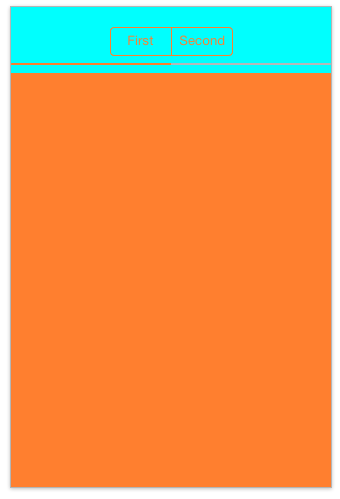
\includegraphics[width=\linewidth, height=\linewidth, keepaspectratio]{img/al_21.png}
\end{minipage}
\begin{minipage}{.5\linewidth}
  \centering
  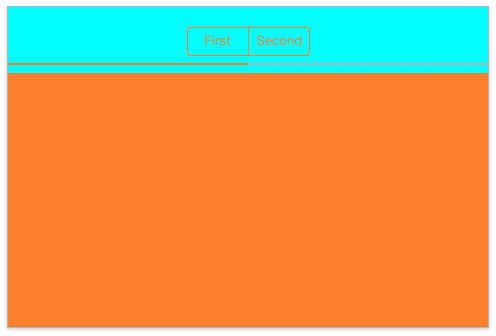
\includegraphics[width=\linewidth, height=\linewidth, keepaspectratio]{img/al_22.png}
\end{minipage}

\item Zwei Buttons im Abstand von 20pt sind am oberen Bildschirmrand zusammen horizontal zentriert. Ein \objcinline{UISlider} mit zugehörigem Label und eine füllende View befinden sich darunter. Ändern wir den Text der Label, passt sich das Layout an.

\begin{minipage}{.5\linewidth}
  \centering
  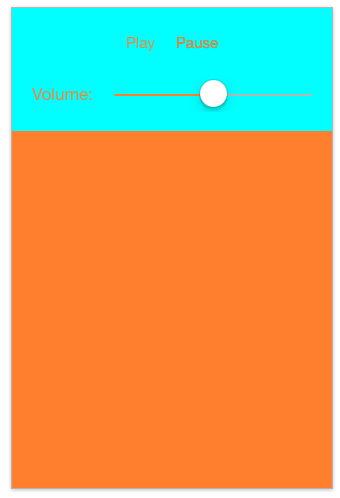
\includegraphics[width=\linewidth, height=\linewidth, keepaspectratio]{img/al_31.png}
\end{minipage}
\begin{minipage}{.5\linewidth}
  \centering
  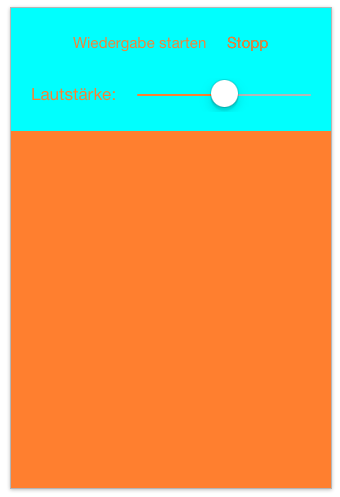
\includegraphics[width=\linewidth, height=\linewidth, keepaspectratio]{img/al_32.png}
\end{minipage}

\item Zwei Views haben (Platzhalter-) Intrinsic Content Sizes von 300x300pt und 100x100pt. Die größere wird wenn möglich vertikal zentriert, hat jedoch immer einen Abstand von mindestens 20pt zur darunter befindlichen kleineren View. Beide sind horizontal zentriert. Die kleinere View ist außerdem immer mindestens 20pt vom unteren Bildschirmrand entfernt. Wird der verfügbare Platz kleiner, wird die größere View vor der kleineren gestaucht.

\begin{minipage}{.5\linewidth}
  \centering
  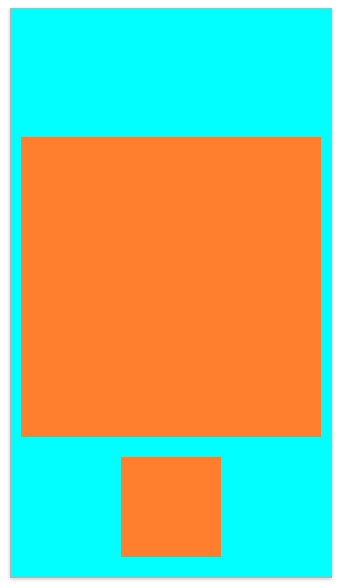
\includegraphics[width=\linewidth, height=\linewidth, keepaspectratio]{img/al_11.png}
\end{minipage}
\begin{minipage}{.5\linewidth}
  \centering
  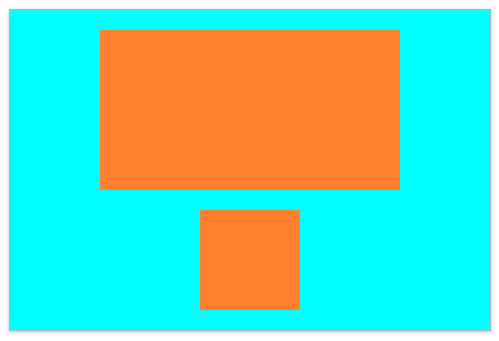
\includegraphics[width=\linewidth, height=\linewidth, keepaspectratio]{img/al_13.png}
\end{minipage}

\item Drei Views füllen jeweils den verfügbaren vertikalen Platz mit einem Abstand von 20pt zur Begrenzung. Horizontal sind sie gleichmäßig verteilt.

\begin{minipage}{.5\linewidth}
  \centering
  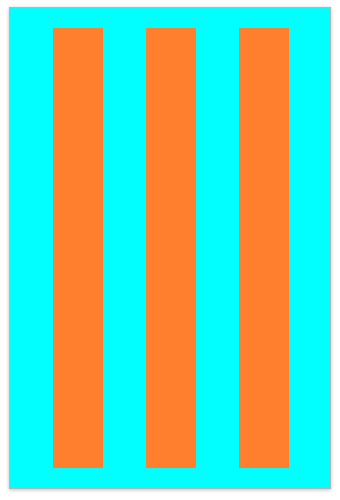
\includegraphics[width=\linewidth, height=\linewidth, keepaspectratio]{img/al_02.png}
\end{minipage}
\begin{minipage}{.5\linewidth}
  \centering
  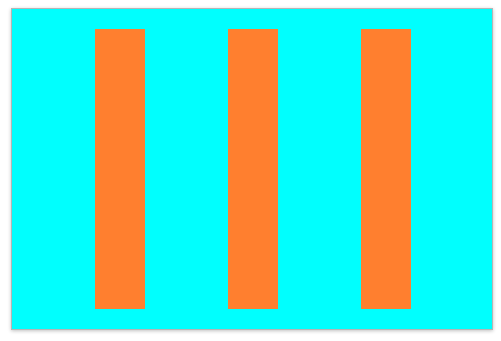
\includegraphics[width=\linewidth, height=\linewidth, keepaspectratio]{img/al_01.png}
\end{minipage}

\end{enumerate}

\end{excitem}

\end{exc}


\end{lecture}


\begin{lecture}


\chapter{Cities}

\mvcindicatorcontroller

iOS Apps bestehen im Allgemeinen nicht nur aus einer, sondern aus einer Vielzahl von untereinander verbundenen Bildschirmansichten. Wir haben gelernt, dass jede Komponente der Benutzeroberfläche letztendlich von einem \objcinline{UIView} Objekt in der View Hierarchie des übergeordneten \objcinline{UIWindow} Objekts dargestellt wird.

Nun können wir die View Hierarchie einer komplexen App natürlich nicht wie im vorherigen Abschnitt zentral im App Delegate verwalten \excref{exc:view_hierarchy}. Um eine sinnvolle Struktur zu schaffen, implementieren wir stattdessen \strong{View Controller}.

Diese sind der Controller-Komponente des Model-View-Controller Konzepts zugeordnet und im Skript ausführlich beschrieben.

Mit dieser App lernen wir das \strong{View Controller Containment} Prinzp kennen, schreiben eigene \objcinline{UIViewController} Subklassen und verwenden einige wichtige View Controller aus dem UIKit Framework.

\skriptref{View Controller Hierarchie}

\section{One City}

Wir wollen zunächst einen Buttons mit dem Titel einer Stadt implementieren und Informationen über die entsprechende Stadt in einem separaten View Controller anzeigen, wenn der Benutzer auf den Button drückt.

\begin{enumerate}

\item Beginnen wir mit einem neuen Xcode Projekt nach dem \emph{Single View} Template und mit dem Product Name \emph{cities}. Es wird damit automatisch eine Klasse \objcinline{AppDelegate} und ein Storyboard hinzugefügt. Zusätzlich befindet sich bereits eine Subklasse \objcinline{ViewController : UIViewController} in unserem Projekt.

\item Die Klasse \objcinline{ViewController} möchten wir zunächst in \objcinline{CitiesViewController} umbenennen. Dazu verwenden wir Xcode's \strong{Refactor} Funktion. Markiert den Namen der Klasse an einer beliebigen Stelle im Code und wählt mit einem Rechtsklick im Kontextmenü \menu{Refactor > Rename...} \abbref{img:refactor}. Geben wir nun den Namen \objcinline{CitiesViewController} ein und bestätigen den Dialog, benennt Xcode das Symbol an allen Stellen im Code, in Storyboards und in Dateinamen um.

\includegraphicsc[8cm]{img/refactor.png}{img:refactor}{Die Refactor Funktion ist sinnvoll, um Symbole im gesamten Projekt umzubennen}

\item Im Storyboard finden wir eine Scene mit einem Objekt dieser (nun umbenannten) \objcinline{CitiesViewController} Klasse. Wie im Skript dargestellt, können wir uns im Identity Inspector davon überzeugen, dass die Klasse des View Controller Objekts tatsächlich \objcinline{CitiesViewController} ist. Zur Laufzeit wird also ein solches Objekt erzeugt und dem \objcinline{UIWindow} Objekt als Root View Controller zugeordnet, da die Scene als \emph{Initial Scene} gekennzeichnet ist. Damit wird die Content View dieses View Controllers zu Beginn der Ausführung der App der View Hierarchie des \objcinline{UIWindow} Objekts hinzugefügt.

\item Ziehen wir nun \objcinline{UIView} Objekte auf die Content View des View Controllers, werden diese zur View Hierarchie der Content View hinzugefügt. Der View Controller ist für die Verwaltung seiner Content View zuständig. Daher stellen wir Verbindungen in Form von IBOutlets und IBActions her, um Zugriff auf die Objekte zu erhalten und um auf Benutzereingaben reagieren zu können.

Wir benötigen zunächst nur ein \objcinline{UIButton} Objekt mit entsprechendem IBOutlet, das den Namen einer beliebigen Stadt anzeigen soll \abbref{img:one_city_ui}. Als Titel des Buttons könnt ihr auch zunächst generisch \emph{City name} o.ä. wählen, da wir diesen im Code anpassen.

\includegraphicsc[\iphonewidth]{img/one_city_ui.png}{img:one_city_ui}{Ein Button soll bei Betätigung Informationen über die entsprechende Stadt anzeigen}

\item Obwohl wir uns in dieser App hauptsächlich mit der Controller-Komponente beschäftigen, sollten wir eine einfache Datenstruktur implementieren, die zu unserer App passt. So können wir Daten einfacher verarbeiten und weitergeben. Erstellt eine neue Klasse \objcinline{City : NSObject} und definiert die Attribute \objcinline{NSString *name} und \objcinline{UIImage *image}.

\begin{objccode}
// City.h

@interface City : NSObject

@property (strong, nonatomic) NSString *name;
@property (strong, nonatomic) UIImage *image;

@end
\end{objccode}

\begin{objccode}
// City.m

#import "City.h"

@implementation City

@end
\end{objccode}

\item Später wird der Cities View Controller eine Liste von Städten anzeigen, doch zunächst beschränken wir uns auf eine. Fügt daher ein Attribut \objcinline{City *city} im öffentlichen Interface hinzu.

\begin{objccode}
// CitiesViewController.h

@class City; // Forward Declaration

@interface CitiesViewController : UIViewController

^\objcinlinehighlight{@property (strong, nonatomic) City *city;}^

@end
\end{objccode}

\item Wir verwenden nun das App Delegate, um zu Beginn der Ausführung der App das Model, also die \objcinline{City} Objekte, aufzusetzen und an die View Controller weiterzugeben. Implementiert daher folgende \objcinline{application:didFinishLaunchingWithOptions:} Methode.

\begin{objccode}
// AppDelegate.m

#import "AppDelegate.h"
#import "City.h"
#import "CitiesViewController.h"

@implementation AppDelegate

- (BOOL)application:(UIApplication *)application didFinishLaunchingWithOptions:(NSDictionary *)launchOptions
{
    City *city = [[City alloc] init];
    city.name = @"Melbourne";
    city.image = [UIImage imageNamed:@"melbourne"];

    CitiesViewController *citiesVC = self.window.rootViewController;
    citiesVC.city = city;
    
    return YES;
}

@end
\end{objccode}

Es gibt natürlich auch Städte in Mittelerde, Panem und auf Naboo…

\strong{Hinweis:} Die Klassenmethode \objcinline{imageNamed:} von \objcinline{UIImage} lädt die Bilddatei mit dem angegebenen Dateinamen, sofern die Datei im Target referenziert ist. Für Dateien im PNG Format muss die Dateiendung nicht enthalten sein. Um dem Target eine Bilddatei hinzuzufügen, könnt ihr sie einfach auf die Dateiliste des Project Navigators ziehen. Praktischer und ressourcenschonender ist jedoch die Verwendung von \strong{Xcode Asset Catalogs} für die Bilddateien einer App. Eine solche mit Dateiendung \emph{.xcassets} ist bereits im Projekt enthalten. Auch dieser Datei könnt ihr per \emph{Drag \& Drop} Bilddateien hinzufügen.

\item Im Cities View Controller überschreiben wir die \objcinline{viewWillAppear:} Methode, um das Interface entsprechend des \objcinline{City} Objekts zu konfigurieren.

\begin{objccode}
// CitiesViewController.m

#import "CitiesViewController.h"
#import "City.h"

@interface CitiesViewController ()

@property (strong, nonatomic) IBOutlet UIButton *cityButton;

@end

@implementation CitiesViewController

- (void)viewWillAppear:(BOOL)animated
{
    [super viewWillAppear:animated];
    
    [self.cityButton setTitle:self.city.name forState:UIControlStateNormal];
}

@end
\end{objccode}

\item Um nun einen Bildschirm zu präsentieren, der die Informationen der ausgewählten Stadt anzeigt, implementieren wir eine weitere Subklasse von \objcinline{UIViewController}. Erstellt also eine neue Klasse \objcinline{CityDetailViewController : UIViewController}. Dieser Klasse übergeben wir das ausgewählte \objcinline{City} Objekt und überlassen ihr die Konfiguration ihrer Content View entsprechend den Attributen des Objekts. Definiert also wieder ein Attribut \objcinline{City *city} im Header der \objcinline{CityDetailViewController} Klasse.

\begin{objccode}
// CityDetailViewController.h

@class City; // Forward Declaration

@interface CityDetailViewController : UIViewController

^\objcinlinehighlight{@property (strong, nonatomic) City *city;}^

@end
\end{objccode}

\item Nun verwenden wir wieder das Storyboard, um die Benutzerführung zu konfigurieren. Zieht ein View Controller Objekt aus der Object Library auf das Storyboard und platziert es neben dem Cities View Controller. Wählt nun im Identity Inspector des hinzugefügten View Controllers das Eingabefeld \emph{Class} und gebt den Namen der neuen \objcinline{UIViewController} Subklasse \objcinline{CityDetailViewController} ein.

\item Platziert ein \objcinline{UILabel} und ein \objcinline{UIImageView} Objekt in der Content View des \objcinline{CityDetailViewController} und verbindet sie mit IBOutlets im Code \abbref{img:city_detail_ui}. Fügt außerdem einen \emph{Zurück} Button hinzu.

\includegraphicsc[\iphonewidth]{img/city_detail_ui.png}{img:city_detail_ui}{Der City Detail View Controller soll Information über die ausgewählte Stadt anzeigen}

\begin{objccode}
// CityDetailViewController.m

#import "CityDetailViewController.h"

@interface CityDetailViewController ()

^\objcinlinehighlight{@property (strong, nonatomic) IBOutlet UILabel *nameLabel;}^
^\objcinlinehighlight{@property (strong, nonatomic) IBOutlet UIImageView *imageView;}^

@end
\end{objccode}

\item Zur Präsentation des City Detail View Controllers können wir nun \strong{Segues} verwenden. Diese repräsentieren, wie im Skript beschrieben, Beziehungen zwischen einzelnen Scenes im Storyboard. Segues können analog zu IBOutlets und IBActions erstellt werden, indem eine Verbindungslinie mit gedrückter \keys{\ctrl}-Taste gezogen wird. Wählt den Button im Cities View Controller aus und zieht eine Verbindung zum City Detail View Controller \abbref{img:one_city_detail_segue}. Erstellt so eine \strong{Modal Segue} zwischen Button und View Controller. 

\includegraphicsc{img/one_city_detail_segue.png}{img:one_city_detail_segue}{Eine Modal Segue konfiguriert die Präsentation des City Detail View Controllers bei Betätigung des Buttons}

Im Attributes Inspector könnt ihr die Segue konfigurieren und bspw. zwischen verschiedenen Übergangsanimationen auswählen. Hier kann außerdem ein \emph{Identifier} für die Segue vergeben werden. Setzt diesen auf \emph{showCityDetail}.

\item Dem erstellten City Detail View Controller muss vor der Präsentation ein \objcinline{City} Objekt übergeben werden, damit er dessen Attribute darstellen kann. Dazu implementieren wir die Instanzmethode \objcinline{prepareForSegue:sender:} in unserer \objcinline{CitiesViewController} Klasse.

\begin{objccode}
// CitiesViewController.m

#import "CitiesViewController.h"
#import "City.h"
#import "CityDetailViewController.h"

@interface CitiesViewController ()

@property (strong, nonatomic) IBOutlet UIButton *cityButton;

@end

@implementation CitiesViewController

- (void)viewWillAppear:(BOOL)animated
{
    [super viewWillAppear:animated];
    
    [self.cityButton setTitle:self.city.name forState:UIControlStateNormal];
}

^\objcinlinehighlight{- (void)prepareForSegue:(UIStoryboardSegue *)segue sender:(id)sender}^
{
    if ([segue.identifier isEqualToString:@"showCityDetail"]) {
        CityDetailViewController *cityDetailVC = segue.destinationViewController;
        cityDetailVC.city = self.city;
    }
}

@end
\end{objccode}

Hier geben wir das \objcinline{City} Objekt also einfach an den City Detail View Controller weiter.

\item Schließlich müssen wir den City Detail View Controller für die Darstellung der Attribute des \objcinline{City} Objekts konfigurieren. Dies geschieht am besten in einer weiteren Implementierung der \objcinline{viewWillAppear:} Instanzmethode in der \objcinline{CityDetailViewController} Klasse.

\begin{objccode}
#import "CityDetailViewController.h"
#import "City.h"

@interface CityDetailViewController ()

@property (strong, nonatomic) IBOutlet UILabel *nameLabel;
@property (strong, nonatomic) IBOutlet UIImageView *imageView;

@end

@implementation CityDetailViewController

- (void)viewWillAppear:(BOOL)animated
{
    [super viewWillAppear:animated];
    
    ^\objcinlinehighlight{self.nameLabel.text = self.city.name;}^
    ^\objcinlinehighlight{self.imageView.image = self.city.image;}^
}

@end
\end{objccode}

Betätigt ihr nun den Button, wird die Content View des City Detail View Controller angezeigt und mit dem entsprechenden \objcinline{City} Objekt konfiguriert \abbref{img:one_city_run}.

\includegraphicsc[\iphonewidth]{img/one_city_run.png}{img:one_city_run}{Wird der Button betätigt, zeigt der City Detail View Controller die Informationen zu der ausgewählten Stadt}

\item Nun fehlt nur noch die Implementierung des \emph{Zurück} Buttons. Hier verwenden wir das Konzept der \strong{Unwind Segue}, um zu einem View Controller in der View Controller Hierarchie zurückzukehren. Dazu fügen wir \emph{dem präsentierenden View Controller} (nicht dem \emph{präsentierten}) eine Methode \objcinline{unwindToCities:} nach dem im Skript beschriebenen Muster hinzu, sodass sie im Interface Builder zur Verfügung steht.

\begin{objccode}
// CitiesViewController.m

#import "CitiesViewController.h"
#import "City.h"
#import "CityDetailViewController.h"

@interface CitiesViewController ()

^\objcinlinehighlight{- (IBAction)unwindToCities:(UIStoryboardSegue *)segue;}^

@end

@implementation CitiesViewController

- (void)prepareForSegue:(UIStoryboardSegue *)segue sender:(id)sender
{
    if ([segue.identifier isEqualToString:@"showCityDetail"]) {
        City *city = [[City alloc] init];
        city.name = @"Melbourne";
        city.image = [UIImage imageNamed:@"melbourne"];
        CityDetailViewController *cityDetailVC = segue.destinationViewController;
        cityDetailVC.city = city;
    }
}

^\objcinlinehighlight{- (IBAction)unwindToCities:(UIStoryboardSegue *)segue}^
{
    // no implementation necessary
}

@end
\end{objccode}

\item Im Storyboard können wir nun das \objcinline{UIControlEventTouchUpInside} Event des \emph{Zurück} Buttons mit der Unwind Segue verbinden. Zieht dazu bei gehaltener \keys{\ctrl}-Taste eine Verbindung vom Button zur \emph{Exit} Schaltfläche des City Detail View Controllers (also des \emph{präsentierten} View Controllers) \abbref{img:cities_unwind_segue}. Da ein View Controller in der View Controller Hierarchie eine Unwind Segue \objcinline{unwindToCities:} implementiert, könnt ihr diese hier auswählen.

\includegraphicsc[\iphonewidth]{img/cities_unwind_segue.png}{img:cities_unwind_segue}{Die \emph{Exit} Schaltfläche präsentiert alle Unwind Segues in der View Controller Hierarchie}

Führt ihr die App nun aus und betätigt den \emph{Zurück} Button, so wird die Unwind Segue zum Cities View Controller ausgeführt und damit der City Detail View Controller wieder ausgeblendet.

\end{enumerate}

\begin{exc}
\begin{excitem}{cities}{Cities}

Implementiert diesen ersten Teil der Cities App, indem ihr die Schritte oben nachvollzieht.

\end{excitem}
\end{exc}


\end{lecture}


\begin{lecture}


\section{One City Navigation}

UIKit stellt für diese häufig verwendete Master-Detail View Controller Hierarchie die Subklasse \objcinline{UINavigationController : UIViewController} zur Verfügung. Diese wird im Skript erläutert und eignet sich an dieser Stelle besser als Modal Segues.

\begin{enumerate}

\item Zieht einfach ein \objcinline{UINavigationController} Objekt aus der Object Library auf euer Storyboard. Dabei wird zusätzlich zu der Navigation Controller Scene automatisch eine weitere View Controller Scene als Root View Controller des Navigation Controllers hinzugefügt. Löscht diesen zusätzlichen View Controller und wählt stattdessen den \objcinline{CitiesViewController} als Root View Controller. Erstellt dafür eine \strong{Relationship Segue} zwischen beiden Objekten, indem ihr wieder mit gedrückter \keys{\ctrl}-Taste eine Verbindung zieht. Markiert außerdem den Navigation Controller als Initial View Controller \abbref{img:nav_controller_segue}.

\includegraphicsc{img/nav_controller_segue.png}{img:nav_controller_segue}{Eine Relationship Segue markiert den Root View Controller eines Navigation Controllers}

\item Ihr könnt nun die Modal Segue zwischen \objcinline{CitiesViewController} und \objcinline{CityDetailViewController} auswählen und im Attributes Inspector den Typ zu \strong{Push Segue} ändern. Nun wird automatisch statt der \objcinline{presentViewController:animated:completion} Methode von \objcinline{UIViewController} die \objcinline{pushViewController:animated:} Methode von \objcinline{UINavigationController} aufgerufen, wenn die Segue ausgelöst wird.

\item Den \emph{Zurück} Button könnt ihr nun entfernen, da \objcinline{UINavigationController} einen eigenen Mechanismus implementiert und eine \objcinline{UINavigationBar} am oberen Bildschirmrand anzeigt. Auch die Labels werden nicht mehr benötigt. Stattdessen können wir das \objcinline{NSString *title} Attribut von \objcinline{UIViewController} verwenden, dessen Wert als Titel in der Navigation Bar angezeigt wird \abbref{img:nav_controller_ui}.

\includegraphicsc{img/nav_controller_ui.png}{img:nav_controller_ui}{Navigation Controller zeigen eine Navigation Bar an}

\begin{objccode}
// CityDetailViewController.m

#import "CityDetailViewController.h"
#import "City.h"

@interface CityDetailViewController ()

@property (strong, nonatomic) IBOutlet UIImageView *imageView;

@end

@implementation CityDetailViewController

- (void)viewWillAppear:(BOOL)animated {
    [super viewWillAppear:animated];
    ^\objcinlinehighlight{self.navigationItem.title = self.city.name;}^
    self.imageView.image = self.city.image;
}

@end
\end{objccode}

Verwendet außerdem gerne Auto Layout, um die Views zu positionieren.

\item Da wir den Initial View Controller und damit den Root View Controller des Window Objekts verändert haben, müssen wir noch kurz die Implementierung des App Delegates anpassen, um das City Objekt korrekt weiterzugeben.

\begin{objccode}
// App Delegate.m > application:didFinishLaunchingWithOptions:
CitiesViewController *citiesVC = (CitiesViewController *)[(UINavigationController *)self.window.rootViewController topViewController];
\end{objccode}


\item Durch die Verwendung des Navigation Controllers erhält unsere App nun die Standardanimationen und -mechanismen aus UIKit, die sich bspw. durch die Verwendung von Subklassen und sog. Delegates vielseitig anpassen lassen \abbref{img:nav_controller_run}.

\includegraphicsc[\iphonewidth]{img/nav_controller_run.png}{img:nav_controller_run}{Navigation Controller stellen Standardanimationen und -mechanismen zur Verfügung}

\end{enumerate}


\section{More Cities}

Wenn wir eine Liste von Objekten darstellen wollen, konfigurieren wir natürlich nicht explizit Views für jedes Objekt. Stattdessen verwenden wir Subklassen von \objcinline{UITableViewController : UIViewController} und ihre Content Views der Klasse \objcinline{UITableView : UIView}, die mit dem \strong{Delegate Konzept} vielseitig einsetzbar sind.

\skriptref{Das Delegate Konzept, Table Views \& Table View Controller}

\begin{enumerate}

\item Wir möchten nun eine Liste von Städten anstatt einzelner Buttons anzeigen. Dafür ändern wir die Superklasse unseres \objcinline{CitiesViewController} von \objcinline{UIViewController} zu \objcinline{UITableViewController}. Außerdem können wir die IBOutlet Referenz zu dem \emph{cityButton} entfernen.

\item Ein Table View Controller hat ein Objekt der \objcinline{UITableView} Klasse als Content View. Im Storyboard müssen wir daher die bisherige Content View mit einem Table View Objekt aus der Object Library ersetzen. Die Content View wird ersetzt, wenn wir die neue View einfach auf das View Controller Objekt in der Document Outline links ziehen.

\strong{Hinweis:} Anstatt einen existierenden View Controller wie beschrieben in einen Table View Controller umzukonfigurieren, kann auch ein Table View Controller aus der Object Library gezogen werden. Dieser hat dann bereits eine \objcinline{UITableView} als Content View

\item Eine Table View kann, wie im Skript beschrieben, dynamischen oder statischen Inhalt darstellen. Im Attributes Inspector können wir den Modus \emph{Dynamic Properties} auswählen. Damit die Table View nun Inhalt präsentieren kann, benötigt sie \strong{Prototype Cells}, die den "{}Bauplan"{} für jede Zelle dieser Art definieren. Fügt dafür eine \objcinline{UITableViewCell} aus der Object Library hinzu oder erhöht die entsprechende Zahl im Attributes Inspector um 1.

\item Wir können Prototype Cells nun entweder nach Belieben mit Subviews konfigurieren, oder im Attributes Inspector einen Standardstil auswählen. Wählt hier zunächst einfach \emph{Basic} \abbref{img:morecities_prototypecells}.

\includegraphicsc[\iphonewidth]{img/morecities_prototypecells.png}{img:morecities_prototypecells}{Prototype Cells dienen als Vorlage für die Zellen der Table View}

\item Um Prototype Cells zu identifizieren, sollte ihnen ein \strong{Reuse Identifier} im Attributes Inspector zugeordnet werden. Tippt hier \emph{cityCell} ein. Wie im Skript erklärt kann die Table View damit Zellen, die gerade nicht angezeigt werden, an anderer Stelle wiederverwenden.

\item Da unsere Table View dynamischen Inhalt anzeigen soll, können wir diesen nicht im Storyboard konfigurieren. Stattdessen verwendet die Table View das \strong{Delegate Kozept}, um Daten zu "{}erfragen"{}, wenn sie sie benötigt. Dazu ruft das \objcinline{UITableView} Objekt Methoden auf einem Delegate Objekt auf, die in einem \strong{Protokoll} definiert sind. \objcinline{UITableView} teilt diese Anfragen in die \objcinline{UITableViewDatasource} und \objcinline{UITableViewDelegate} Protokolle auf. Um den entsprechenden Attributen \objcinline{id<UITableViewDatasource> datasource} und \objcinline{id<UITableViewDelegate> delegate} Objekte zuzuweisen, sind diese als IBOutlets markiert. Zieht also zwei Verbindungen von der Table View zum \objcinline{CitiesViewController} und wählt diesen damit sowohl als Delegate als auch als Datasource.

\item Im Allgemeinen repräsentiert eine Table View ein \objcinline{NSArray}. Definiert also im öffentlichen Interface des \objcinline{CitiesViewController} ein Attribut \objcinline{NSArray *cities} anstatt des bisherigen \objcinline{City *city} Attributs.

\begin{objccode}
// CitiesViewController.h

@interface CitiesViewController : UITableViewController

^\objcinlinehighlight{@property (strong, nonatomic) NSArray *cities;}^

@end
\end{objccode}

Passt außerdem erneut die Implementierung des App Delegates an, um diesem Attribut nun eine Liste von Städten zuzuweisen.

\begin{objccode}
// AppDelegate.m

- (BOOL)application:(UIApplication *)application didFinishLaunchingWithOptions:(NSDictionary *)launchOptions
{
    // create some city objects
    City *melbourne = [[City alloc] init];
    melbourne.name = @"Melbourne";
    melbourne.image = [UIImage imageNamed:@"melbourne"];
    City *sydney = [[City alloc] init];
    sydney.name = @"Sydney";
    sydney.image = [UIImage imageNamed:@"sydney"];
    // (...)

    // provide root view controller with model objects
    CitiesViewController *citiesVC = (CitiesViewController *)[(UINavigationController *)self.window.rootViewController topViewController];
    citiesVC.cities = @[melbourne, sydney];
    
    return YES;
}

\end{objccode}

\item Als Subklasse von \objcinline{UITableViewController} erbt \objcinline{CitiesViewController} leere Implementierungen der \objcinline{UITableViewDatasource} und \objcinline{UITableViewDelegate} Protokolle. Wir können diese nun überschreiben, um unsere Tabelle mit Daten zu füllen. Dabei sind zunächst die drei erforderlichen Methoden zur Darstellung einer dynamischen Table View zu implementieren:

\begin{objccode}
#pragma mark - Table View Datasource

- (NSInteger)numberOfSectionsInTableView:(UITableView *)tableView {
    return 1;
}

- (NSInteger)tableView:(UITableView *)tableView numberOfRowsInSection:(NSInteger)section {
    return [self.cities count];
}

- (UITableViewCell *)tableView:(UITableView *)tableView cellForRowAtIndexPath:(NSIndexPath *)indexPath {

    // Greift auf das Model zurück, um das darzustellende Objekt zu erhalten
    City *city = [self.cities objectAtIndex:indexPath.row];

    // Erstellt ein neues UITableViewCell Objekt entsprechend der im Storyboard definierten Prototype Cell mit dem gegebenen Identifier oder verwendet eine existierende, momentan nicht verwendete Zelle mit diesem Identifier
    UITableViewCell *cell = [tableView dequeueReusableCellWithIdentifier:@"cityCell" forIndexPath:indexPath];

    // Konfiguriert die View entsprechend des Models
    cell.textLabel.text = city.name;
    cell.imageView.image = city.image;

    return cell;
}
\end{objccode}

\objcinline{#pragma mark} kennzeichnet eine Überschrift ähnlich eines Kommentars und wird zusätzlich in der Jump Bar angezeigt. Ein Bindestrich \objcinline{-} erzeugt dort eine horizontale Trennlinie.

Die zuvor implementierten Methoden werden nicht mehr benötigt.

\item Diese drei Methoden des \objcinline{UITableViewDatasource} Protokolls stellen der Table View die erforderlichen Informationen zur Verfügung, um die Tabelle anzeigen zu können \abbref{img:cities_tableview}.

\includegraphicsc[\iphonewidth]{img/cities_tableview.png}{img:cities_tableview}{Eine Table View stellt Anfragen an ihr Datasource und Delegate Objekt, um Zellen dynamisch anzuzeigen}

\item Die Präsentation des Detail City View Controllers kann nun erneut mithilfe von Segues realisiert werden. Dazu können wir im Storyboard eine Push Segue von der Prototype Cell zum Detail City View Controller erstellen und ihr erneut den Identifier \emph{showCityDetail} geben.

\item Da diese Segue nun von jeder Zelle ausgelöst wird, die nach Vorlage der Prototype Cell erstellt wurde, müssen wir in der \objcinline{prepareForSegue:sender:} Methode zunächst den Index Path der betätigten Zelle herausfinden. Damit lässt sich anschließend das entsprechende Model Objekt erhalten und der City Detail View Controller konfigurieren.

\begin{objccode}
//  ViewController.m

#import "CitiesViewController.h"
#import "City.h"
#import "CityDetailViewController.h"

@implementation CitiesViewController

#pragma mark - User Interaction

- (void)prepareForSegue:(UIStoryboardSegue *)segue sender:(id)sender
{
    if ([segue.identifier isEqualToString:@"showCityDetail"]) {

        City *city = [self.cities objectAtIndex:self.tableView.indexPathForSelectedRow.row];
        
        CityDetailViewController *cityDetailVC = segue.destinationViewController;
        cityDetailVC.city = city;
    }
}

#pragma mark - Table View Datasource

// (...)

@end
\end{objccode}

\item Wird nun eine Stadt in der Liste ausgewählt, wird der City Detail View Controller entsprechend konfiguriert und angezeigt. Beachtet, dass wir an dessen Implementierung nichts geändert haben!

\end{enumerate}

\begin{exc}

\begin{excitem}{tableviews}{Cities 2}

Implementiert die Cities App nun vollständig, indem ihr die Schritte oben nachvollzieht.

\end{excitem}

\end{exc}


\end{lecture}


\begin{lecture}


\chapter{Seasonizer}

Mit den Apps der vergangenen Vorlesungen haben wir die Grundlagen der Programmierung für iOS Geräte und einige wichtige Architekturkonzepte kennengelernt. Mit diesem Wissen lässt sich bereits ein Großteil der zur Verfügung stehenden Frameworks anwenden und viele Funktionen, die iOS Geräte bieten, in unsere eigenen Apps integrieren.

%Aus gegebenem Anlass implementieren wir in dieser App einige häufig verwendete Funktionen wie Multi-Touch Gesten und Kamera Integration, um beim nächsten Familienfest nicht nur mit unseren neu erworbenen Programmierfähigkeiten anzugeben, sondern auch noch Fotos von Familienmitgliedern festlich dekorieren zu können \abbref{img:seasonizer}.

Zusammenfassend implementieren wir in dieser App einige häufig verwendete Funktionen wie Multi-Touch Gesten und Kamera Integration, um beim nächsten Familienurlaub nicht nur mit unseren neu erworbenen Programmierfähigkeiten anzugeben, sondern auch noch Fotos von Familienmitgliedern sommerlich dekorieren zu können \abbref{img:seasonizer}.

\includegraphicsc[\iphonewidth]{img/seasonizer_summer.png}{img:seasonizer}{Mit der Seasonizer App lassen sich Familienmitglieder dekorieren und ungewollte Haarfarben verdecken}

\subsubsection{Funktionen der Seasonizer App}

\emph{Das Sternsystem kennzeichnet die Schwierigkeit der Funktion von * (machbar) bis *** (unmöglich).}

\begin{description}
\item [*] Die App besitzt eine Hauptansicht mit Navigation Bar und Toolbar. Den Inhalt füllt eine Image View für das Foto und eine darüberliegende View mit transparentem Hintergrund für die Accessories.
\item [*] Es gibt einen Button in der Toolbar, mit dem ein Foto von der Kamera oder Foto Bibliothek ausgewählt werden kann, das anschließend von der Image View angezeigt wird.
\item [**] Ein weiterer Button zeigt modal eine Liste von Accessories an. Wird ein Accessory ausgewählt, wird es der Hauptansicht hinzugefügt.
\item [**] Die Accessories lassen sich mit Gesten verschieben, skalieren, drehen und löschen.
\item [*] Mit einem Action Button kann das Bild über verschiedene Kanäle wie Nachrichten, Email oder Facebook verteilt werden.
\item [**] Die Elemente wie Bild und Accessories werden gespeichert und beim nächsten Start der App wiederhergestellt.
\item [*] Ein Toolbar Button dient dem Zurücksetzen der Benutzeroberfläche.
%\item [extra] Es schneit in der App!
\item [extra] Es regnet in der App! Das passiert ja auch mal.
\item [extra] Implementiert, was euch einfällt! Ich bin auf eure Ideen gespannt.
\end{description}

Anders als für die bisherigen Apps wird es an dieser Stelle keine vollständige Schritt-für-Schritt Anleitung geben. Versucht stattdessen, die Funktionen der App zu implementieren, indem ihr die folgenden Hinweise und die Informationen der bisherigen Themen anwendet. Ich stehe dabei natürlich jederzeit gerne für Fragen zur Verfügung.

\subsubsection{Hinweise}

\begin{itemize}

\item Wenn ihr mit dem \emph{Single View} Template beginnt, bietet es sich an, dem View Controller der Hauptansicht mithilfe der \emph{Refactor} Funktion einen sinnvollen Namen wie \objcinline{CanvasViewController} zu geben. Verwendet außerdem den Project Name \emph{seasonizer}.

\item \strong{Navigation Bar und Toolbar} lassen sich sehr einfach anzeigen, wenn ein Navigation Controller verwendet wird. Buttons lassen sich dann als Objekte der \objcinline{UIBarButtonItem} Klasse aus der Object Library dem Navigation Item hinzufügen. \objcinline{UIBarButtonItem} bietet bereits viele Stile wie \objcinline{UIBarButtonSystemItemCamera} zur Auswahl im Attributes Inspector an.

\item Die Auswahl zwischen \strong{Kamera und Foto Bibliothek} lässt sich sinnvoll mit einem \objcinline{UIActionSheet} implementieren:

\begin{objccode}
- (IBAction)cameraButtonPressed:(id)sender {
    UIActionSheet *actionSheet = [[UIActionSheet alloc] initWithTitle:nil delegate:self cancelButtonTitle:@"Abbrechen" destructiveButtonTitle:nil otherButtonTitles:@"Kamera", @"Foto Bibliothek", nil];
    [actionSheet showFromToolbar:self.navigationController.toolbar];
}
\end{objccode}

Der View Controller muss nun als Empfänger des \objcinline{UIActionSheetDelegate} Protokolls markiert werden und die Delegate Methode \objcinline{actionSheet:clickedButtonAtIndex:} implementieren. Hier können wir einen \objcinline{UIImagePickerController} anzeigen, der als \objcinline{UIImagePickerControllerSourceTypeCamera} oder \objcinline{UIImagePickerControllerSourceTypePhotoLibrary} konfiguriert werden kann.

\begin{objccode}
- (void)actionSheet:(UIActionSheet *)actionSheet clickedButtonAtIndex:(NSInteger)buttonIndex {
    if (buttonIndex==actionSheet.cancelButtonIndex) return;
    
    // Der erste Button zeigt die Kamera, der zweite die Photo Library
    UIImagePickerControllerSourceType sourceType = (buttonIndex==actionSheet.firstOtherButtonIndex) ? UIImagePickerControllerSourceTypeCamera : UIImagePickerControllerSourceTypePhotoLibrary;
    
    // Für Geräte ohne Kamera muss die Verfügbarkeit des Source Types getestet werden
    if (![UIImagePickerController isSourceTypeAvailable:sourceType]) {
        UIAlertView *alertView = [[UIAlertView alloc] initWithTitle:@"Option nicht verfügbar" message:@"Dieses Gerät unterstützt diese Option nicht." delegate:nil cancelButtonTitle:@"Ok" otherButtonTitles:nil];
        [alertView show];
        return;
    }
    
    // Den UIImagePickerController erstellen, konfigurieren und anzeigen
    UIImagePickerController *imagePickerC = [[UIImagePickerController alloc] init];
    imagePickerC.delegate = self;
    imagePickerC.sourceType = sourceType;
    [self presentViewController:imagePickerC animated:YES completion:nil];
}
\end{objccode}

Der \objcinline{UIImagePickerController} verwendet abermals das Delegate Konzept, also muss der View Controller nun außerdem als Empfänger des \objcinline{UIImagePickerControllerDelegate} Protokolls markiert werden und folgende Methoden implementieren:

\begin{objccode}
- (void)imagePickerController:(UIImagePickerController *)picker didFinishPickingMediaWithInfo:(NSDictionary *)info {
    [picker dismissViewControllerAnimated:YES completion:nil];
    
    self.photoImageView.image = [info objectForKey:UIImagePickerControllerOriginalImage];
    
}
- (void)imagePickerControllerDidCancel:(UIImagePickerController *)picker {
    [picker dismissViewControllerAnimated:YES completion:nil];
}
\end{objccode}

\item Wir arbeiten in dieser App mit \strong{Accessory Objekten}, die jeweils ein Bild repräsentieren und Eigenschaften wie Titel haben können. Daher bietet es sich an, eine Klasse \objcinline{Accessory : UIImageView} zu erstellen. Objekten dieser Klasse erben dann die Darstellungsmechanismen der \objcinline{UIImageView} Klasse und es können Attribute wie \objcinline{NSString *title} hinzugefügt werden.

\item Um modal einen weiteren View Controller mit Titelleiste für die \strong{Accessory Liste} anzuzeigen, kann dieser wiederum in einem Navigation Controller verpackt werden \abbref{img:seasonizer_ui}. Es sollte eine dynamische Table View in einer Subklasse \objcinline{AccessoryListViewController : UITableViewController} verwendet werden, um die Liste der verfügbaren Accessories anzuzeigen.

\includegraphicsc{img/seasonizer_ui.png}{img:seasonizer_ui}{Navigation Controller bieten eine einfache Möglichkeit, Navigationsleisten und Toolbars anzuzeigen}

\item Der Accessory List View Controller kann ein privates Attribut \objcinline{NSArray *accessories} mit überschriebener Getter Methode implementieren, das der dynamischen Table View als Informationsquelle dient.

\begin{objccode}
- (NSArray *)accessories {
    if (!_accessories) {
        
        Accessory *sunglasses = [[Accessory alloc] init];
        sunglasses.title = @"Sonnenbrille";
        sunglasses.image = [UIImage imageNamed:@"sunglasses"];

        Accessory *sunhat = [[Accessory alloc] init];
        sunhat.title = @"Sonnenhut";
        sunhat.image = [UIImage imageNamed:@"sunhat"];

        // ...
        
        _accessories = @[sunglasses, sunhat];
    }
    return _accessories;
}
\end{objccode}

\item Ihr könnt Bilddateien entweder direkt ins Projekt ziehen und damit referenzieren, oder \strong{Asset Catalogs} verwenden. Im Projekt befindet sich bereits eine \emph{.xcassets} Datei, in der leere Referenzen zu App Icon und Launch Image zu finden sind. Hier könnt ihr einfach weitere Bilddateien auf den linken Listenbereich bewegen. Ein \strong{Image Set} besteht dabei immer aus einer Bilddatei mit normaler und einer mit doppelter Auflösung für Geräte mit Retina Display. Abhängig vom ausführenden Gerät wird hier immer die korrekte Datei geladen. Dies funktioniert ebenfalls für referenzierte Bilddateien außerhalb von Asset Catalogs, die wie \emph{image.png} und \emph{image@2x.png} benannt sind.

\item Die Auswahl eines Accessories kann mithilfe eines eigenen Delegate Protokolls implementiert werden. Dazu benötigt der Accessory List View Controller ein öffentliches Attribut \objcinline{id <AccessorySelectionDelegate> delegate} und sollte das Protokoll in seinem Header definieren:

\begin{objccode}
// AccessoryListViewController.h

@class Accessory; // Forward Declaration
@protocol AccessorySelectionDelegate; // Forward Declaration

@interface AccessoryListViewController : UITableViewController

@property (weak, nonatomic) id <AccessorySelectionDelegate> delegate;

@end

@protocol AccessorySelectionDelegate

- (void)accessoryListViewController:(AccessoryListViewController *)accessoryListVC didSelectAccessory:(Accessory *)accessory;

@end
\end{objccode}

Nun kann das Delegate Objekt über die Auswahl eines Accessories informiert werden:

\begin{objccode}
// in AccessoryListViewController.m

- (void)tableView:(UITableView *)tableView didSelectRowAtIndexPath:(NSIndexPath *)indexPath {
    Accessory *accessory = [self.accessories objectAtIndex:indexPath.row];

    [self.delegate accessoryListViewController:self didSelectAccessory:accessory];
    
}
\end{objccode}

Wenn der Canvas View Controller den Accessory View Controller präsentiert, muss er dem \objcinline{delegate} Attribut zugewiesen werden:

\begin{objccode}
// in CanvasViewController.m

- (void)prepareForSegue:(UIStoryboardSegue *)segue sender:(id)sender {
    if ([segue.identifier isEqualToString:@"showAccessoryList"]) {
        // Der Accessory List View Controller ist nicht das direkte Ziel der Segue, sondern dessen Navigation Controller. Daher müssen wir dessen Top View Controller verwenden, der nun der Accessory List View Controller ist.
        AccessoryListViewController *accessoryListVC = (AccessoryListViewController *)[segue.destinationViewController topViewController];
        accessoryListVC.delegate = self;
    }
}
\end{objccode}

Der Canvas View Controller muss nun außerdem als Empfänger des \objcinline{AccessorySelectionDelegate} Protokolls markiert werden und dieses implementieren:

\begin{objccode}
// in CanvasViewController.m

- (void)accessoryListViewController:(AccessoryListViewController *)accessoryListVC didSelectAccessory:(Accessory *)accessory {
    
    [self addAccessory:accessory]; // Diese Methode muss noch implementiert werden
    
    // Passe initiale Position und Größe an
    [accessory sizeToFit];
    accessory.center = [accessory.superview convertPoint:accessory.superview.center fromView:accessory.superview.superview];

    [accessoryListVC dismissViewControllerAnimated:YES completion:nil];
}
\end{objccode}

\item Der Canvas View Controller kann die angezeigten Accessories mit einem Attribut \objcinline{NSMutableArray *accessories} verwalten. Dafür sollte er zwei Methoden \objcinline{addAccessory:} und \objcinline{removeAccessory:} implementieren:

\begin{objccode}
- (void)addAccessory:(Accessory *)accessory {
    if (!self.accessories) self.accessories = [[NSMutableArray alloc] init];
    
    [self.accessories addObject:accessory]; // add accessory to list
    [self.accessoryView addSubview:accessory]; // display accessory on screen
    
}

- (void)removeAccessory:(Accessory *)accessory {
    [accessory removeFromSuperview];
    [self.accessories removeObject:accessory];
}
\end{objccode}

\item Für die Manipulation der Accessories mit Gesten können wir \strong{Gesture Recognizer} verwenden. UIKit implementiert einige hilfreiche Subklassen von \objcinline{UIGestureRecognizer}, die bestimmt Multi-Touch Events auf der ihr zugewiesenen View erkennen und ihr Delegate Objekt darüber informieren. Also können wir den Canvas View Controller als Empfänger des \objcinline{UIGestureRecognizerDelegate} Protokolls markieren, Gesture Recognizer in der \objcinline{addAccessory:} Methode hinzufügen und die Delegate Methoden zum Bewegen, Skalieren, Rotieren und Löschen der Accessories implementieren.

\begin{objccode}
- (void)addAccessory:(Accessory *)accessory {
    if (!self.accessories) self.accessories = [[NSMutableArray alloc] init];
    
    [self.accessories addObject:accessory];
    [self.accessoryView addSubview:accessory];

    accessory.userInteractionEnabled = YES; // UIImageView empfängt im Allgemeinen keine Touch Events, daher müssen wir dies hier aktivieren

    // Bewegen
    UIPanGestureRecognizer *panGR = [[UIPanGestureRecognizer alloc] initWithTarget:self action:@selector(pan:)];
    panGR.delegate = self;
    [accessory addGestureRecognizer:panGR];
    
    // Skalieren
    UIPinchGestureRecognizer *pinchGR = [[UIPinchGestureRecognizer alloc] initWithTarget:self action:@selector(pinch:)];
    pinchGR.delegate = self;
    [accessory addGestureRecognizer:pinchGR];

    // Drehen
    UIRotationGestureRecognizer *rotateGR = [[UIRotationGestureRecognizer alloc] initWithTarget:self action:@selector(rotate:)];
    rotateGR.delegate = self;
    [accessory addGestureRecognizer:rotateGR];

    // Löschen
    UILongPressGestureRecognizer *tapGR = [[UILongPressGestureRecognizer alloc] initWithTarget:self action:@selector(tap:)];
    tapGR.delegate = self;
    [accessory addGestureRecognizer:tapGR];
    
}

#pragma mark Gestures

- (BOOL)gestureRecognizer:(UIGestureRecognizer *)gestureRecognizer shouldRecognizeSimultaneouslyWithGestureRecognizer:(UIGestureRecognizer *)otherGestureRecognizer {
    // Gesture Recognizer unterbrechen die Erkennung einer Geste bei der Erkennung einer anderen, wenn hier NO zurückgegeben wird. 
    return YES;
}

- (void)pan:(UIPanGestureRecognizer *)sender {
    [sender.view.superview bringSubviewToFront:sender.view];
    
    CGPoint translation = [sender translationInView:sender.view.superview];
    sender.view.center = CGPointMake(sender.view.center.x+translation.x, sender.view.center.y+translation.y);

    [sender setTranslation:CGPointZero inView:sender.view.superview];
}

- (void)pinch:(UIPinchGestureRecognizer *)sender {
    [sender.view.superview bringSubviewToFront:sender.view];
    
    sender.view.transform = CGAffineTransformScale(sender.view.transform, sender.scale, sender.scale);
    
    [sender setScale:1.];
}

- (void)rotate:(UIRotationGestureRecognizer *)sender {
    [sender.view.superview bringSubviewToFront:sender.view];

    sender.view.transform = CGAffineTransformRotate(sender.view.transform, sender.rotation);
    
    [sender setRotation:0.];
}

- (void)tap:(UILongPressGestureRecognizer *)sender {
    if (sender.state!=UIGestureRecognizerStateBegan) return;
    
    [self becomeFirstResponder];
    UIMenuController *menuController = [UIMenuController sharedMenuController];
    [menuController setMenuItems:@[[[UIMenuItem alloc] initWithTitle:@"Entfernen" action:@selector(removeAccessoryButtonPressed:)]]];
    [menuController setTargetRect:CGRectMake(sender.view.center.x, sender.view.center.y, 0, 0) inView:sender.view.superview];
    [menuController setMenuVisible:YES animated:YES];

    tappedAccessory = (Accessory *)sender.view;
}
- (BOOL)canBecomeFirstResponder {
    return YES;
}

- (void)removeAccessoryButtonPressed:(id)sender {
    [self removeAccessory:tappedAccessory];
}
\end{objccode}

Hier sei angemerkt, dass wir aufgrund des Zusammenspiels verschiedener Gesture Recognizer jeweils Delta-Bewegungen verwenden und auf die View anwenden, indem der jeweilige Gesture Recognizer bei jedem Methodenaufruf zurückgesetzt wird.

Der \objcinline{UILongPressGestureRecognizer} zeigt einen speziellen \objcinline{UIMenuController} zur Darstellung eines \emph{Entfernen} Buttons. Damit dieser korrekt angezeigt wird, muss die \objcinline{canBecomeFirstResponder} Methode implementiert werden. Außerdem müssen wir eine Referenz auf das entsprechende \objcinline{Accessory} Objekt zwischenspeichern, um es in der Action Methode weiterverwenden zu können. Dazu kann dem Klasseninterface ein Attribut oder, wie hier gezeigt, eine Instanzvariable hinzugefügt werden:

\begin{objccode}
@interface CanvasViewController () < /* viele Protokolle */ > {
    
    Accessory *tappedAccessory; // Instanzvariable
    
}

// Attribut- und Methodendefinitionen ...

@end

\end{objccode}

\item Die Integration eines \strong{Activity Sheets} zum Teilen von Inhalten ist denkbar einfach. UIKit stellt dafür den \objcinline{UIActivityViewController} zur Verfügung, der eine Liste von Datenobjekten annimmt und abhängig vom Typ der Daten eine Auswahl von Kanälen zum Teilen anzeigt.

\begin{objccode}
- (IBAction)actionButtonPressed:(id)sender {
    UIActivityViewController *activityVC = [[UIActivityViewController alloc] initWithActivityItems:@[self.renderedPicture] applicationActivities:nil];
    [self presentViewController:activityVC animated:YES completion:nil];
}
\end{objccode}

In dieser Methode wird auf die Getter Methode eines Attributs \objcinline{UIImage *renderedPicture} zugegriffen. Dieses Attribut soll dazu dienen, auf das vollständige Bild zugreifen zu können. Es soll dieses aber nicht speichern, sondern bei jedem Aufruf neu generieren, da das Bild sich natürlich ändern kann. Also markieren wir das Attribut bei der Definition als \objcinline{readonly} und überschreiben dessen Getter Methode:

\begin{objccode}
// im Header
@property (readonly) UIImage *renderedPicture;
\end{objccode}

\begin{objccode}
// in der Implementierung
- (UIImage *)renderedPicture {
    UIGraphicsBeginImageContextWithOptions(self.canvasView.frame.size, YES, 0.);
    [self.canvasView drawViewHierarchyInRect:self.canvasView.bounds afterScreenUpdates:YES];
    UIImage *renderedPicture = UIGraphicsGetImageFromCurrentImageContext();
    UIGraphicsEndImageContext();
    return renderedPicture;
}
\end{objccode}

Hier wurde \objcinline{canvasView} im Storyboard als Superview der Image View (für das Foto) und der Accessory View (für die Accessories) konfiguriert.

\item Als kleines Extra können wir es in der App regnen lassen. Für graphische Spielereien dieser Art müssen wir etwas weiter in die Trickkiste greifen und mit dem \strong{Core Animation} Framework arbeiten. Fügt dem Projekt einfach eine Bilddatei \emph{raindrop.png} mit etwa 15x15 Pixelmaßen hinzu und verwendet folgenden Code:

\begin{objccode}
// in CanvasViewController.m

- (void)viewDidLoad {
    [super viewDidLoad];

    CAEmitterCell *cell = [CAEmitterCell emitterCell];
    
    cell.name = @"raindrop";
    cell.birthRate = 50.;
    cell.velocity = 250.;
    cell.velocityRange = cell.velocity / 2.;
    cell.yAcceleration = 10.;
    cell.emissionLongitude = M_PI_2;
    cell.contents = (id)[UIImage imageNamed:@"raindrop"].CGImage;
    cell.lifetime = 7.;
    cell.alphaRange = 1.;
    cell.alphaSpeed = -1./cell.lifetime;
    
    CAEmitterLayer *emitter = [CAEmitterLayer layer];
    [emitter setEmitterCells:@[cell]];
    [emitter setFrame:self.navigationController.view.bounds];
    [emitter setEmitterPosition:CGPointMake(self.navigationController.view.bounds.size.width/2, -15.)];
    [emitter setEmitterSize:CGSizeMake(self.navigationController.view.frame.size.width, 0.)];
    [emitter setEmitterShape:kCAEmitterLayerRectangle];
    [emitter setRenderMode:kCAEmitterLayerAdditive];
    [self.navigationController.view.layer addSublayer:emitter];
    
}
\end{objccode}

\item Um die Benutzeroberfläche vollständig wiederherstellen zu können, müssen wir sowohl das Foto als auch die hinzugefügten Accessories speichern. Als Methode der Datenspeicherung bietet sich in dieser App die \strong{User Defaults} Mechanik an, doch auch das \strong{State Preservation} System könnte stattdessen verwendet werden.

Zur Speicherung der Accessories müssen wir in der \objcinline{Accessory : UIImageView} Klasse zunächst das \objcinline{NSCoding} Protokoll implementieren. Dieses Protokoll bietet die Möglichkeit, Objekte als \objcinline{NSData} zu serialisieren. \objcinline{UIImageView} implementiert dieses Protokoll bereits, daher müssen wir in der Subklasse lediglich die beiden Schlüsselmethoden überschreiben:

\begin{objccode}
- (void)encodeWithCoder:(NSCoder *)aCoder
{
    [super encodeWithCoder:aCoder];
    
    // encode properties
    [aCoder encodeObject:self.title forKey:@"title"];
}

- (id)initWithCoder:(NSCoder *)aDecoder
{
    if ((self = [super initWithCoder:aDecoder])) {
    
        // decode properties
        self.title = [aDecoder decodeObjectForKey:@"title"];
        
    }
    return self;
}
\end{objccode}

Nun können wir das \strong{Notifications} System verwenden, um über die Veränderung des App States informiert zu werden. Bewegt sich die App in den Hintergrund, sollen Bild und Accessories in den User Defaults gespeichert werden. In der \objcinline{viewDidLoad} Methode des Canvas View Controllers fügen wir diesen daher als Empfänger der \objcinline{UIApplicationDidEnterBackgroundNotification} hinzu und implementieren eine Methode, die bei Empfang einer solchen Notification aufgerufen wird:

\begin{objccode}
- (void)viewDidLoad
{
    [super viewDidLoad];
    
    [[NSNotificationCenter defaultCenter] addObserver:self selector:@selector(didEnterBackground:) name:UIApplicationDidEnterBackgroundNotification object:[UIApplication sharedApplication]];
    
    // ...
}

#define kUserDefaultsKeyPhotoImage @"image_data"
#define kUserDefaultsKeyAccessories @"accessory_data"

- (void)didEnterBackground:(NSNotification *)notification
{
    NSData *imageData = UIImagePNGRepresentation(self.photoImageView.image);
    [[NSUserDefaults standardUserDefaults] setObject:imageData forKey:kUserDefaultsKeyPhotoImage];

    NSData *accessoryData = [NSKeyedArchiver archivedDataWithRootObject:self.accessories]; // NSArray und alle enthaltenen Objekte der Klasse Accessory implementieren das NSCoding Protokoll und können somit archiviert werden
    [[NSUserDefaults standardUserDefaults] setObject:accessoryData forKey:kUserDefaultsKeyAccessories];
}
\end{objccode}

Die Wiederherstellung dieser gesicherten Daten kann nun in der \objcinline{viewDidLoad} Methode erfolgen:

\begin{objccode}
- (void)viewDidLoad
{
    [super viewDidLoad];
        
    NSData *imageData = [[NSUserDefaults standardUserDefaults] objectForKey:kUserDefaultsKeyPhotoImage];
    self.photoImageView.image = [UIImage imageWithData:imageData];
    
    NSData *accessoryData = [[NSUserDefaults standardUserDefaults] objectForKey:kUserDefaultsKeyAccessories];
    NSArray *accessories = [NSKeyedUnarchiver unarchiveObjectWithData:accessoryData];
    for (Accessory *accessory in accessories) {
        [self addAccessory:accessory];
    }
    
    // ...
}
\end{objccode}

Hier verwenden wir die \objcinline{addAccessory:} Methode, um die Accessories der View Hierarchie hinzuzufügen und die Gesture Recognizer zu erzeugen. In der vorherigen Version dieses Dokuments wurde in der \objcinline{addAccessory:} Methode außerdem die Position und Größe des neuen Accessories angepasst. Dies kann jedoch stattdessen in der Delegate Methode \objcinline{accessoryListViewController:didSelectAccessory:} geschehen. Beide Methoden sind oben in der veränderten Form zu finden.

\item Implementieren wir einen weiteren Toolbar Button, der die Benutzeroberfläche bei Betätigung \strong{zurücksetzt}, sollte zunächst eine Schaltfläche zur Bestätigung erscheinen.

Dazu eignet sich wieder ein \objcinline{UIActionSheet}. Dieses muss jedoch in der Implementierung der Delegate Methoden von dem Action Sheet zur Auswahl zwischen Kamera und Fotobibliothek unterschieden werden. Eine Möglichkeit besteht in der Definition eines privaten Attributs für jedes der beiden Action Sheets in der \objcinline{CanvasViewController} Klasse. Dann können wir die Action Methode des Reset Buttons wie folgt implementieren:

\begin{objccode}
- (IBAction)resetButtonPressed:(id)sender
{
    UIActionSheet *actionSheet = [[UIActionSheet alloc] initWithTitle:nil delegate:self cancelButtonTitle:@"Abbrechen" destructiveButtonTitle:@"Zurücksetzen" otherButtonTitles:nil];
    self.resetActionSheet = actionSheet; // dient der Identifikation des Action Sheets in der Delegate Methode
    [actionSheet showFromToolbar:self.navigationController.toolbar];
}
\end{objccode}

Analog muss die \objcinline{cameraButtonPressed:} Methode um die Attributzuweisung \objcinline{self.photoActionSheet = actionSheet} erweitert werden.

In der \objcinline{UIActionSheetDelegate} Methode \objcinline{actionSheet:clickedButtonAtIndex:} können wir nun eine Fallunterscheidung zwischen den Action Sheets durchführen:

\begin{objccode}
- (void)actionSheet:(UIActionSheet *)actionSheet clickedButtonAtIndex:(NSInteger)buttonIndex
{
    if (buttonIndex==actionSheet.cancelButtonIndex) return;
    
    if (actionSheet==self.resetActionSheet&&buttonIndex==actionSheet.destructiveButtonIndex)         {
        
        [self resetCanvas]; // muss noch implementiert werden
        
    } else if (actionSheet==self.photoActionSheet) {
        
        // ...
        
    }
}
\end{objccode}

In einer Methode \objcinline{resetCanvas} kann die Benutzeroberfläche dann zurückgesetzt werden:

\begin{objccode}
- (void)resetCanvas
{
    self.photoImageView.image = nil;
    
    [self.accessories makeObjectsPerformSelector:@selector(removeFromSuperview)];
    self.accessories = nil;
}
\end{objccode}

\end{itemize}


\subsubsection{Der Seasonizer auf GitHub}

Auf GitHub findet ihr eine Beispielimplementierung des Seasonizers \linkref{https://github.com/iOS-Dev-Kurs/seasonizer}, die ihr als Referenz verwenden und auch weiterentwickeln könnt.

Anstatt mein Repository direkt lokal zu klonen, könnt ihr mit eurem eigenen GitHub Account den Fork Button \linkref{https://github.com/iOS-Dev-Kurs/seasonizer/fork} meines Repositories klicken. Damit wird das Repository serverseitig unter eurem Account geklont. Ihr könnt es nun auf eurem Account finden und lokal klonen:

\begin{shcode}
cd path/to/directory
git clone https://github.com/yourusername/seasonizer
\end{shcode}

Hier könnt ihr nun Commits durchführen und diese mit eurer serverseitigen Kopie meines Repositories abgleichen.

\begin{shcode}
# add commits ...
git push
\end{shcode}

Haltet ihr eure Änderungen für so genial oder notwendig, dass sie in mein Original Repository übernommen werden sollten, könnt ihr mir über die GitHub Webseite eine \strong{Pull Request} schicken, die mich auffordert, einen Merge mit den Änderungen durchzuführen.

Andere Entwickler, die mein Repository geklont haben, können diese Änderungen anschließend herunterladen. In dieser Form kann ein Open Source Programmierprojekt weltweit von interessierten Entwicklern weiterentwickelt werden. Und dem Seasonizer sind damit keine Grenzen gesetzt.


\end{lecture}


\end{document}
